% =============================================================================
%  Capítulo 5. Desarrollo
% =============================================================================

\chapter{Desarrollo}
\label{cap:desarrollo}

En este capítulo se detalla la implementación del sistema, organizada en torno a
los flujos de datos que lo recorren de extremo a extremo. Se parte de una visión
global por capas (sección~\ref{sec:vision-flujos}) y, a continuación, se desciende
al detalle de la infraestructura de despliegue (sección~\ref{sec:infraestructura}),
del backend (sección~\ref{sec:backend}), de la capa robótica
(sección~\ref{sec:capa-robotica}) y de la aplicación de usuario
(sección~\ref{sec:app-usuario}). La descripción se ancla en el código fuente del
proyecto, del que se incluyen extractos representativos.

% =============================================================================
\section{Vista general y flujos de datos}
\label{sec:vision-flujos}

El sistema se estructura en seis capas, desde la aplicación de usuario hasta la
plataforma física del robot. La figura~\ref{fig:arquitectura} las presenta
apiladas, junto con los componentes que las integran. El flujo de información es
bidireccional: las órdenes del usuario descienden desde la aplicación hasta la
plataforma física, mientras que la telemetría y las incidencias ascienden en
sentido contrario.

% ---------------------------------------------------------------------------
\begin{figure}[H]
  \centering
  \usetikzlibrary{arrows.meta}%
  \begin{tikzpicture}[
      capa/.style={align=center, text width=0.86\linewidth, inner sep=3pt},
      flecha/.style={-{Stealth[length=2.4mm]}, line width=0.7pt, draw=black!75},
      node distance=6mm
    ]
    \def\titulo{\bfseries}%
    \def\comp{\footnotesize\color{blue!55!black}}%
    \node[capa] (app) {{\titulo Aplicación de usuario (Flutter)}\\[2pt]
      {\comp Acceso, Inicio, Robots, Incidencias, Perfil, Administración}};
    \node[capa, below=of app] (api) {{\titulo API REST (FastAPI)}\\[2pt]
      {\comp Endpoints de robot, usuario y administración; autenticación JWT}};
    \node[capa, below=of api] (serv) {{\titulo Servicios del backend}\\[2pt]
      {\comp Consumidores de eventos, productor de comandos, lógica de negocio,
        seguridad}};
    \node[capa, below=of serv] (bus) {{\titulo Bus de eventos y almacenes}\\[2pt]
      {\comp Kafka, PostgreSQL, InfluxDB, MinIO, Grafana}};
    \node[capa, below=of bus] (ros) {{\titulo Capa robótica (ROS 2)}\\[2pt]
      {\comp patrol\_nav, detect\_incident, serve\_telemetry, secret\_helper}};
    \node[capa, below=of ros] (fis) {{\titulo Plataforma física}\\[2pt]
      {\comp TurtleBot 4, Nav2, slam\_toolbox, explore\_lite, cámara OAK-D}};
    \foreach \a/\b in {app/api, api/serv, serv/bus, bus/ros, ros/fis} {
      \draw[flecha] ([xshift=-8mm]\a.south) -- ([xshift=-8mm]\b.north); % descendente
      \draw[flecha] ([xshift=8mm]\b.north) -- ([xshift=8mm]\a.south);   % ascendente
    }
    \node[draw=black!75, line width=0.6pt, fit=(app)(fis), inner sep=8pt] {};
  \end{tikzpicture}
  \caption[Arquitectura del sistema por capas]{Vista general del sistema
    organizada en capas, desde la aplicación de usuario hasta la plataforma
    física del robot. Fuente: elaboración propia.}
  \label{fig:arquitectura}
\end{figure}
% ---------------------------------------------------------------------------

Los apartados siguientes describen los tres flujos principales que atraviesan
estas capas.

% ---------------------------------------------------------------------------
\subsection{Cliente \texorpdfstring{$\rightarrow$}{->} servidor
  \texorpdfstring{$\rightarrow$}{->} robot: control de la patrulla}
\label{sec:flujo-control}

Las órdenes del usuario (iniciar, detener y reinstalar la patrulla) viajan desde
la aplicación hasta el robot a través del backend y del bus de eventos. La
aplicación invoca el endpoint correspondiente
(\texttt{PUT /user/\{id\}/start-patrol}, \texttt{stop-patrol} o \texttt{reinstall}).
El backend valida que el robot pertenece al usuario autenticado y que su estado
operativo permite la transición; a continuación publica un comando en el topic
\texttt{robot\_commands} de Kafka. En el robot, el nodo orquestador
\texttt{patrol\_nav} sondea dicho topic cada 0,5\,s
(\texttt{poll\_command\_topic}), descarta los mensajes cuyo \texttt{robot\_id} no
coincide con el suyo y, según el comando, ejecuta \texttt{handle\_start\_patrol},
\texttt{handle\_stop\_patrol} o \texttt{handle\_reinstall}, provocando la
transición de su máquina de estados.

Cada comando responde a una intención del usuario distinta (el detalle de las
transiciones se aborda en la sección~\ref{sec:patrol-nav}). \textbf{Iniciar} pone
en marcha la patrulla (el robot se desacopla de su base antes de moverse): si el robot
no dispone todavía de un mapa, dispara la
exploración y el mapeo del entorno antes de empezar a patrullar; si ya existe un
mapa guardado, lo reutiliza y pasa directamente a planificar la ruta y a recorrerla.
\textbf{Detener} cancela la navegación en curso, devuelve el robot al \textit{dock},
donde se acopla, y deja la patrulla en pausa. \textbf{Reinstalar} borra el mapa guardado y devuelve
el robot a su estado inicial, de modo que el siguiente inicio vuelve a explorar el
entorno desde cero.

Conviene precisar cómo se gobierna el estado en la base de datos. La orden de
inicio no escribe el estado operativo en la base de datos: deja esa
responsabilidad al \textit{heartbeat} del robot, de modo que la primera vuelta no
se salte la fase de mapeo. En cambio, las órdenes de detención y reinstalación sí
fijan de forma optimista los valores \texttt{stopped} e \texttt{idle},
respectivamente. En todos los casos, el \textit{heartbeat} periódico del robot
(sección~\ref{sec:flujo-telemetria}) actúa como fuente de verdad que reconcilia el
estado almacenado con el estado real.

Esta delegación introduce una ventana de consistencia eventual acotada. La
aplicación no realiza una actualización optimista de la interfaz: tras enviar la
orden vuelve a consultar el estado, que puede seguir mostrando el valor previo
hasta que el siguiente \textit{heartbeat} (a lo sumo 10\,s después) actualice la
base de datos y el sondeo periódico de la aplicación (cada 5\,s) lo refleje. Se
trata, por tanto, de un retardo breve y acotado, no de una inconsistencia
permanente, ya que el \textit{heartbeat} garantiza la convergencia al estado real.

% ---------------------------------------------------------------------------
\subsection{Robot \texorpdfstring{$\rightarrow$}{->} servidor
  \texorpdfstring{$\rightarrow$}{->} cliente: telemetría, incidencias y estado}
\label{sec:flujo-telemetria}

En sentido ascendente coexisten tres caminos.

\paragraph*{Telemetría.} El nodo \texttt{serve\_telemetry} publica el estado del
robot una vez por segundo en el topic \texttt{robot\_telemetry}, incorporando el
\gls{jwt} del robot en la cabecera \texttt{Authorization} del mensaje. En el
backend, un consumidor en hilo independiente verifica el token, comprueba que el
\texttt{robot\_id} del mensaje coincide con el del token y escribe un punto de la
medida \texttt{robot\_telemetry} en InfluxDB. Grafana consume esa serie temporal y
la aplicación la muestra empotrada en modo \textit{kiosk}, obteniendo la
\acrshort{url} filtrada por robot mediante \texttt{GET /user/\{id\}/dashboard-url}.

\paragraph*{Incidencias.} El nodo \texttt{detect\_incident} detecta personas
mediante visión por computador, graba un vídeo del suceso, lo sube a MinIO y
publica en el topic \texttt{robot\_incidents} (de nuevo con el \gls{jwt} en
cabecera) los datos del objeto almacenado. El consumidor de incidencias del
backend valida el token, crea un registro \texttt{Incidente} en PostgreSQL y lo
deja disponible para la aplicación, que lista las incidencias
(\texttt{GET /user/incidents}) y reproduce el vídeo a través de una \acrshort{url}
prefirmada (\texttt{GET /user/incidents/\{id\}/show-video}).

\paragraph*{Estado operativo.} El orquestador \texttt{patrol\_nav} envía un
\textit{heartbeat} cada 10\,s mediante \texttt{PUT /robot/heartbeat},
traduciendo su estado interno de la \gls{fsm} a uno de los valores admitidos. El
backend valida el valor recibido y actualiza la conexión y el estado operativo del
robot en PostgreSQL, datos que la aplicación refleja en la pantalla de inicio.

% ---------------------------------------------------------------------------
\subsection{Autenticación y arranque: TOFU y JWT}
\label{sec:flujo-tofu}

Antes de poder emitir telemetría o incidencias, el robot debe autenticarse. El nodo
\texttt{secret\_helper} aplica el patrón \gls{tofu} para acordar un secreto con el
backend en el primer arranque y, a partir de ese secreto, obtener un \gls{jwt} que
renueva de forma periódica. El resto de nodos consume ese token sin gestionar
credenciales por su cuenta. El mecanismo se describe en detalle en la
sección~\ref{sec:secret-helper}.

La tabla~\ref{tab:flujos} resume los flujos descritos.

\begin{table}[htbp]
  \centering
  \small
  \caption{Resumen de los flujos de datos del sistema. Fuente: elaboración propia.}
  \label{tab:flujos}
  \begin{tabular}{@{}>{\raggedright\arraybackslash}p{2.3cm}
                     >{\raggedright\arraybackslash}p{2.8cm}
                     >{\raggedright\arraybackslash}p{5.0cm}
                     >{\raggedright\arraybackslash}p{2.4cm}@{}}
    \toprule
    \textbf{Flujo} & \textbf{Sentido} & \textbf{Recorrido principal} &
    \textbf{Persistencia} \\
    \midrule
    Control de patrulla & App~$\rightarrow$~Robot &
    REST $\rightarrow$~Kafka \texttt{robot\_commands} $\rightarrow$~\gls{fsm} &
    PostgreSQL \\
    \addlinespace[7pt]
    Telemetría & Robot~$\rightarrow$~App &
    Kafka \texttt{robot\_telemetry} $\rightarrow$~InfluxDB $\rightarrow$~Grafana &
    InfluxDB \\
    \addlinespace[7pt]
    Incidencias & Robot~$\rightarrow$~App &
    MinIO + Kafka \texttt{robot\_incidents} $\rightarrow$~\textit{backend} &
    MinIO, PostgreSQL \\
    \addlinespace[7pt]
    Estado operativo & Robot~$\rightarrow$~App &
    \texttt{PUT /robot/heartbeat} & PostgreSQL \\
    \addlinespace[7pt]
    Autenticación & Robot~$\leftrightarrow$~Backend &
    \gls{tofu}: \texttt{first-boot} / \texttt{auth} $\rightarrow$~\gls{jwt} &
    PostgreSQL \\
    \bottomrule
  \end{tabular}
\end{table}

% =============================================================================
\section{Arquitectura e infraestructura}
\label{sec:infraestructura}

La infraestructura se despliega mediante contenedores. El fichero
\texttt{docker-compose.yml} del backend define ocho servicios: la base de datos
relacional (\texttt{postgres}), el bus de eventos (\texttt{zookeeper} y
\texttt{kafka}) con su trabajo de inicialización (\texttt{init-kafka}), la base de
series temporales (\texttt{influxdb}), el almacén de objetos (\texttt{minio}) con
su inicializador (\texttt{init-minio}) y la visualización (\texttt{grafana}). Por
su parte, el \texttt{docker-compose.yml} de \texttt{robot\_ws} define un único servicio de
desarrollo \gls{ros} (\texttt{ros2\_dev}), conectado a la red externa
\texttt{backend\_default}.

Conviene matizar que este \texttt{docker-compose} no constituye el despliegue de
producción del robot, sino un entorno de desarrollo y simulación: proporciona, con
acceso a WSLg y \acrshort{gpu}, las herramientas gráficas (RViz y Gazebo principalmente) necesarias
para ejecutar pruebas y lanzar simulaciones sin depender del hardware. En una
instalación real, los nodos descritos en la sección~\ref{sec:capa-robotica} se
ejecutan directamente sobre la plataforma física del TurtleBot~4.

Es importante señalar que ni el backend (\textit{FastAPI}) ni los nodos del robot
se ejecutan dentro de los contenedores de infraestructura: corren como procesos
externos y se conectan a los servicios anteriores a través de los puertos
publicados en el anfitrión. La tabla~\ref{tab:puertos} recoge esos puertos.

\begin{table}[htbp]
  \centering
  \small
  \caption{Servicios de infraestructura y puertos publicados. Fuente: elaboración propia.}
  \label{tab:puertos}
  \begin{tabular}{@{}>{\raggedright\arraybackslash}p{2.4cm}
                     >{\raggedright\arraybackslash}p{3.2cm}
                     >{\raggedright\arraybackslash}p{2.6cm}
                     >{\raggedright\arraybackslash}p{3.4cm}@{}}
    \toprule
    \textbf{Servicio} & \textbf{Imagen} & \textbf{Puerto} & \textbf{Función} \\
    \midrule
    postgres  & postgres:17                 & 5432         & Datos relacionales \\
    zookeeper & cp-zookeeper:7.5.0           & 2181 (int.)  & Coordinación Kafka \\
    kafka     & cp-kafka:7.5.0               & 9094 / 29092 & Bus de eventos \\
    influxdb  & influxdb:2.7                 & 8086         & Series temporales \\
    minio     & minio (2024)                & 9000 / 9001  & Objetos / consola \\
    grafana   & grafana:latest              & 3000         & Visualización \\
    backend   & FastAPI (proceso)           & 8000         & \gls{api} \gls{rest} \\
    nodos robot & \gls{ros} (procesos)      & n/d          & Cliente del bus \\
    \bottomrule
  \end{tabular}
\end{table}

La topología de red de Kafka merece una nota. El \textit{broker} expone dos
\textit{listeners}: uno interno, en el puerto~29092, para los clientes que viven
dentro de la red de contenedores, y otro externo, en el puerto~9094, para el
backend y los nodos del robot cuando corren en el anfitrión. El
extracto~\ref{lst:kafka} muestra esa configuración, en la que
\texttt{<IP-DEL-HOST>} representa la dirección real del anfitrión. Los trabajos de
inicialización crean, respectivamente, los tres topics
(\texttt{robot\_incidents}, \texttt{robot\_telemetry}, \texttt{robot\_commands}) y
el \textit{bucket} \texttt{tfg-incidentes} de MinIO. Por coherencia, los nodos del
robot disponen de dos ficheros de entorno: \texttt{.env} para ejecución en el
anfitrión y \texttt{.env.container} con las direcciones internas
(\texttt{kafka:29092}, \texttt{minio:9000}, \texttt{host.docker.internal:8000}).

\SuspendTagging{code}%
\begin{yamlcode}[title={Listeners del broker Kafka (docker-compose.yml)}, label={lst:kafka}]
kafka:
  image: confluentinc/cp-kafka:7.5.0
  environment:
    KAFKA_ADVERTISED_LISTENERS: PLAINTEXT://kafka:29092,PLAINTEXT_HOST://<IP-DEL-HOST>:9094
    KAFKA_LISTENER_SECURITY_PROTOCOL_MAP: PLAINTEXT:PLAINTEXT,PLAINTEXT_HOST:PLAINTEXT
    KAFKA_INTER_BROKER_LISTENER_NAME: PLAINTEXT
  ports:
    - "9094:9094"
\end{yamlcode}%
\ResumeTagging{code}

% =============================================================================
\section{Backend}
\label{sec:backend}

El backend, construido con \textit{FastAPI}, expone la \gls{api} \gls{rest},
gestiona la persistencia y aloja los consumidores de eventos. Se organiza en
módulos: \texttt{models.py} (modelo de datos), \texttt{server.py} (endpoints y
consumidores), \texttt{security.py} (criptografía y tokens) y
\texttt{dependencies.py} (inyección de identidad).

% ---------------------------------------------------------------------------
\subsection{Modelo de datos}
\label{sec:modelo-datos}

El modelo, definido con el \gls{orm} \textit{SQLAlchemy} en \texttt{models.py},
consta de tres entidades. \texttt{Usuario} tiene clave primaria entera
autoincremental, \texttt{email} único e indexado, un rol (\texttt{user} o
\texttt{admin}, por defecto \texttt{user}) y la contraseña almacenada como
\texttt{password\_hash}. \texttt{Robot} usa una clave primaria de tipo cadena
(\texttt{String(50)}, apta para números de serie), un \texttt{secret\_hash}
inicialmente nulo (se genera en el primer arranque \gls{tofu}), una clave foránea
\texttt{usuario\_id} hacia su propietario y los campos \texttt{estado\_conexion}
(\texttt{online}/\texttt{offline}) y \texttt{estado\_operativo}; conserva además
marcas temporales de creación y de última actividad, esta última actualizada en cada
escritura mediante \texttt{onupdate}. \texttt{Incidente} emplea como clave primaria un
identificador \texttt{UUID} generado aleatoriamente (\texttt{uuid4}), lo que dificulta
la enumeración de recursos por fuerza bruta, junto con \texttt{bucket\_name},
\texttt{video\_filename} y el indicador \texttt{revisado}.

La elección de los tipos de clave primaria no es accidental: que el usuario tenga un
identificador numérico y el robot una cadena no numérica es lo que permite distinguir
a ambos a partir del sujeto (\texttt{sub}) del token, sin necesidad de un campo de
tipo adicional (sección~\ref{sec:seguridad}). El borrado se propaga en cascada
(\texttt{ondelete=CASCADE}): al eliminar un usuario se eliminan sus robots y, con
ellos, sus incidencias. Para acelerar las consultas más frecuentes, la tabla de
incidencias declara dos índices: uno compuesto por robot y fecha
(\texttt{idx\_incidentes\_robot\_fecha}), que sirve al listado cronológico por robot,
y otro parcial sobre las no revisadas (\texttt{idx\_incidentes\_no\_revisados}, con
condición \texttt{revisado = false}), que se mantiene compacto al cubrir únicamente
las incidencias pendientes de atención.

La persistencia se organiza en torno a \texttt{SessionLocal}, una \textit{fábrica de
sesiones} de \textit{SQLAlchemy} creada con \texttt{sessionmaker}: cada llamada a
\texttt{SessionLocal()} produce una sesión nueva, es decir, una conversación aislada
con la base de datos. Se configura con \texttt{autocommit} y \texttt{autoflush}
desactivados, lo que otorga control explícito sobre la transacción: ningún cambio se
envía ni se confirma de forma implícita, sino solo cuando el código lo ordena con
\texttt{commit}, de modo que una petición que falle a mitad no deja datos a medio
escribir. Para que cada petición \gls{http} disponga de su propia sesión y esta se cierre
siempre al terminar, el acceso se encapsula en la dependencia \texttt{get\_db}, que
\textit{FastAPI} inyecta en cada endpoint que la declara. Los consumidores de eventos,
que viven fuera del ciclo de petición, gestionan su sesión por su cuenta con
\texttt{SessionLocal()}.

% ---------------------------------------------------------------------------
\subsection{API REST}
\label{sec:api-rest}

La tabla~\ref{tab:endpoints} recoge el inventario completo de endpoints, agrupados
según la dependencia de autenticación que exigen, y no según la etiqueta de
documentación, que en algunos casos resulta engañosa.

\begin{table}[htbp]
  \centering
  \small
  \caption[Endpoints de la API REST]{Endpoints de la API REST agrupados por ámbito
  de autenticación. Fuente: elaboración propia. Se omiten los endpoints base
  \texttt{GET /} y \texttt{GET /health}.}
  \label{tab:endpoints}
  \begin{tabular}{@{}>{\ttfamily}l >{\ttfamily}l l@{}}
    \toprule
    \textbf{\normalfont Método} & \textbf{\normalfont Ruta} &
    \textbf{Autenticación} \\
    \midrule
    \multicolumn{3}{@{}l}{\textit{Ámbito robot}} \\
    PUT    & /robot/heartbeat        & JWT robot \\
    POST   & /robot/\{id\}/first-boot & Ninguna (TOFU) \\
    POST   & /robot/\{id\}/auth       & secret\_key \\
    \midrule
    \multicolumn{3}{@{}l}{\textit{Ámbito usuario}} \\
    POST   & /user/register          & Ninguna \\
    POST   & /user/login             & Ninguna \\
    GET    & /user/profile           & JWT usuario \\
    POST   & /user/new-robot         & JWT usuario \\
    GET    & /user/robots            & JWT usuario \\
    DELETE & /user/\{id\}/delete       & JWT usuario \\
    GET    & /user/\{id\}/dashboard-url & JWT usuario \\
    PUT    & /user/\{id\}/start-patrol  & JWT usuario \\
    PUT    & /user/\{id\}/stop-patrol   & JWT usuario \\
    PUT    & /user/\{id\}/reinstall     & JWT usuario \\
    PUT    & /user/\{id\}/alias         & JWT usuario \\
    GET    & /user/incidents         & JWT usuario \\
    GET    & /user/\{id\}/incidents    & JWT usuario \\
    GET    & /user/incidents/\{id\}    & JWT usuario \\
    PUT    & /user/incidents/\{id\}/review & JWT usuario \\
    GET    & /user/incidents/\{id\}/show-video & JWT usuario \\
    PUT    & /user/update-password   & JWT usuario \\
    PUT    & /user/update-info       & JWT usuario \\
    \midrule
    \multicolumn{3}{@{}l}{\textit{Ámbito administración}} \\
    GET    & /admin/robots           & JWT admin \\
    GET    & /admin/robots/\{id\}/incidents & JWT admin \\
    GET    & /admin/incidents/\{id\}   & JWT admin \\
    GET    & /admin/incidents/\{id\}/show-video & JWT admin \\
    PUT    & /admin/incidents/\{id\}/review & JWT admin \\
    GET    & /admin/users            & JWT admin \\
    DELETE & /admin/users/\{id\}/delete & JWT admin \\
    DELETE & /admin/robots/\{id\}/delete & JWT admin \\
    PUT    & /admin/users/\{id\}/grant  & JWT admin \\
    PUT    & /admin/users/\{id\}/revoke & JWT admin \\
    \bottomrule
  \end{tabular}
\end{table}

La autenticación se resuelve por inyección de dependencias de \textit{FastAPI}. Un
esquema \texttt{HTTPBearer} extrae el token de la cabecera \texttt{Authorization} y
tres dependencias lo traducen a identidad: \texttt{get\_current\_user} y
\texttt{get\_current\_robot} decodifican el token y cargan la entidad
correspondiente, mientras que \texttt{get\_current\_admin} encadena la primera y
además exige rol de administrador. Cada endpoint declara la dependencia que necesita,
de modo que el control de acceso queda expresado en la propia firma de la función y
\textit{FastAPI} rechaza la petición antes de ejecutar el cuerpo si la identidad no es
la adecuada.

Los endpoints de control ilustran el patrón completo. \texttt{PUT
/user/\{id\}/start-patrol} comprueba primero que el robot pertenece al usuario
autenticado (en caso contrario responde \texttt{403 Forbidden}) y que su
\texttt{estado\_operativo} admite la transición: solo se puede iniciar desde
\texttt{idle} o \texttt{stopped}, y cualquier otro estado devuelve \texttt{409
Conflict} con un mensaje explicativo. Superadas las validaciones, el endpoint publica
en el topic \texttt{robot\_commands} un mensaje \gls{json} con la estructura
\texttt{\{robot\_id, command, timestamp\}}, usando el \texttt{robot\_id} como clave de
partición y forzando la entrega con \texttt{flush} (tiempo límite de cinco segundos);
si el \textit{broker} no está disponible, responde \texttt{503 Service Unavailable}.
\texttt{stop-patrol} aplica la misma plantilla pero solo admite la transición desde
\texttt{patrolling}, y \texttt{reinstall} no impone restricción de estado.

Aquí se materializa la asimetría descrita en la sección~\ref{sec:flujo-control}. En
\texttt{start-patrol}, la línea que escribiría el estado en la base de datos se ha
dejado deliberadamente comentada en el código: tras
publicar el comando en Kafka, el endpoint devuelve el robot sin tocar su
\texttt{estado\_operativo}, de manera que sea el \textit{heartbeat} quien refleje la
progresión real \texttt{exploring}~$\rightarrow$~\dots~$\rightarrow$~\texttt{patrolling}
y la primera vuelta no se salte la fase de mapeo. En cambio, \texttt{stop-patrol} y
\texttt{reinstall} sí fijan de forma optimista \texttt{stopped} e \texttt{idle},
respectivamente, porque son estados terminales que no dependen de un proceso ulterior
del robot.

Dos endpoints de lectura completan el flujo del usuario. \texttt{GET
/user/\{id\}/dashboard-url} construye, tras validar la propiedad del robot, la
\acrshort{url} del panel de Grafana en modo \textit{kiosk} filtrada por el robot
(\texttt{var-robot\_id}), con ventana temporal de las últimas seis horas y refresco
cada diez segundos. \texttt{GET /user/incidents/\{id\}/show-video} genera con
\textit{boto3} una \acrshort{url} prefirmada del objeto de MinIO con validez de una hora
(\texttt{ExpiresIn=3600}), de manera que la aplicación reproduce el vídeo sin exponer
las credenciales del almacén ni hacer público el \textit{bucket}.

% ---------------------------------------------------------------------------
\subsection{Consumidores y productor de eventos}
\label{sec:consumidores}

En \texttt{server.py}, la función \texttt{create\_server\_consumers} instancia dos
consumidores de Kafka y un productor para los comandos. Cada consumidor pertenece a
un grupo propio (\texttt{incident-consumer} y \texttt{telemetry-consumer}) y difiere
en su política de \textit{offset} inicial, una decisión deliberada: el de incidencias
arranca desde el mensaje más antiguo (\texttt{auto.offset.reset = earliest}) para no
perder ningún suceso aunque el servidor haya estado caído, mientras que el de
telemetría arranca desde el más reciente (\texttt{latest}), porque una medida atrasada
carece de valor y solo interesa el estado actual del robot.

Al iniciarse el servidor, cada bucle de consumo arranca en un hilo \textit{daemon}
independiente (extracto~\ref{lst:consumers}), de modo que la espera de mensajes no
bloquea al hilo principal que atiende las peticiones \gls{http} y los consumidores se
detienen solos al apagar el servidor. El productor de comandos se guarda en
\texttt{app.state} para que lo compartan los endpoints de control.

Cada mensaje recibido pasa por la misma cadena de validación antes de procesarse
(sección~\ref{sec:seguridad}): se verifica el \gls{jwt} de la cabecera y se comprueba
que el \texttt{robot\_id} del cuerpo coincide con el sujeto del token, descartando el
mensaje en cualquier otro caso.

\SuspendTagging{code}%
\begin{pythoncode}[title={Consumidores en hilos daemon y sondeo del broker (server.py)}, label={lst:consumers}]
# Distinta politica de offset inicial por consumidor.
incident_consumer = Consumer({
    'bootstrap.servers': settings.kafka_broker_url,
    'group.id': 'incident-consumer',
    'auto.offset.reset': 'earliest'})   # No perder sucesos pasados.
telemetry_consumer = Consumer({
    'bootstrap.servers': settings.kafka_broker_url,
    'group.id': 'telemetry-consumer',
    'auto.offset.reset': 'latest'})     # Solo interesa el estado actual.

# Cada bucle corre en un hilo daemon: no bloquea el apagado ni las peticiones HTTP.
threading.Thread(target=detect_incident,
                 args=(incident_consumer,), daemon=True).start()
threading.Thread(target=serve_telemetry,
                 args=(telemetry_consumer,), daemon=True).start()

# Dentro de cada bucle: espera <= 1 s por mensaje, sin espera activa.
while True:
    msg = consumer.poll(1.0)
    if msg is None:
        continue                        # No habia mensajes en este intervalo.
    # ... validacion del JWT y del robot_id antes de procesar ...
\end{pythoncode}%
\ResumeTagging{code}

El tratamiento posterior difiere según el flujo. El consumidor de telemetría compone
un punto de la medida \texttt{robot\_telemetry}, etiquetado por \texttt{robot\_id} y
con los campos de estado del robot (batería y voltaje, posición, velocidades lineal y
angular, e indicadores de atraque, secuestro, deslizamiento y ruedas), y lo escribe en
InfluxDB con la marca temporal que envía el propio robot, a precisión de nanosegundos.
El consumidor de incidencias abre una sesión de base de datos por mensaje, inserta una
fila \texttt{Incidente} con los datos del objeto almacenado y confirma la transacción,
revirtiéndola si se produce un error. Al apagarse, \texttt{shutdown\_event} vacía el
productor para no perder los comandos pendientes de entrega.

% ---------------------------------------------------------------------------
\subsection{Seguridad}
\label{sec:seguridad}

La seguridad se apoya en varios mecanismos complementarios concentrados en
\texttt{security.py} y \texttt{dependencies.py}. El esquema parte de una premisa: el
robot opera sin supervisión y no puede depender de que una persona introduzca
credenciales, de modo que acuerda un secreto con el backend en su primer contacto
(\gls{tofu}) y, a partir de él, porta su identidad en cada petición y evento mediante
un \gls{jwt}. Las contraseñas de usuario y los
secretos de robot nunca se almacenan en claro: se cifran de forma irreversible con
\textit{bcrypt} a través de \textit{passlib} (un \texttt{CryptContext} con el esquema
\texttt{bcrypt}), que incorpora \textit{salt} y un factor de coste configurable. El
secreto raíz del robot, base del \gls{tofu}, se genera con el módulo \texttt{secrets}
de Python como una cadena aleatoria de treinta y dos caracteres alfanuméricos con un
prefijo identificativo (\texttt{rbt\_sec\_}), y de él solo se persiste el \textit{hash}.

La identidad se transporta en \gls{jwt} firmados con el algoritmo simétrico HS256. El
\textit{payload} contiene únicamente el sujeto (\texttt{sub}) y la fecha de expiración
(\texttt{exp}), fijada por defecto a 1440 minutos (veinticuatro horas). La función
\texttt{verificar\_token} valida la firma y la vigencia y traduce los fallos a
respuestas \texttt{401}, distinguiendo el token caducado
(\texttt{ExpiredSignatureError}) del inválido o corrupto (\texttt{InvalidTokenError}).
La distinción entre usuarios y robots se resuelve sin almacenar el tipo: se observa si
el sujeto del token es numérico, ya que los identificadores de usuario lo son y los de
robot (cadenas) no. Sobre esta base, \texttt{get\_current\_user} rechaza con
\texttt{403} un token cuyo sujeto no sea numérico y \texttt{get\_current\_robot} hace
lo contrario, evitando que una credencial de robot opere como usuario o viceversa. El
control de acceso por roles (\gls{rbac}) se aplica en \texttt{get\_current\_admin}, que
encadena la verificación de usuario y exige rol de administrador; además, los endpoints
de administración protegen contra operaciones peligrosas sobre la propia cuenta (un
administrador no puede borrarse ni revocarse a sí mismo).

Para los mensajes que llegan por Kafka, que no atraviesan las dependencias de
\textit{FastAPI}, el backend replica la verificación en el propio bucle de consumo:
valida el \gls{jwt} incluido en la cabecera del mensaje y comprueba que el
\texttt{robot\_id} del cuerpo coincide con el sujeto del token, evitando la
suplantación de un robot por otro. El acceso a los vídeos se realiza mediante
\acrshort{url} prefirmadas de MinIO generadas con \textit{boto3} y caducidad de una hora,
de modo que el \textit{bucket} permanece privado. Conviene señalar de forma explícita
una limitación conocida: la política de \gls{cors} permanece abierta en el estado
actual del desarrollo y debe restringirse antes de un despliegue en producción. El
extracto~\ref{lst:jwt} muestra la generación y verificación de tokens.

\SuspendTagging{code}%
\begin{pythoncode}[title={Generación y verificación de JWT (security.py)}, label={lst:jwt}]
def generate_jwt_token(subject: str) -> str:
    tiempo_expiracion = datetime.now(timezone.utc) + timedelta(
        minutes=settings.access_token_expire_minutes)
    payload = {"sub": str(subject), "exp": tiempo_expiracion}
    return jwt.encode(payload, settings.secret_key,
                      algorithm=settings.algorithm)

def verificar_token(token: str) -> str:
    payload = jwt.decode(token, settings.secret_key,
                         algorithms=[settings.algorithm])
    subject = payload.get("sub")
    if not subject:
        raise HTTPException(status_code=401, detail="Token sin ID (subject)")
    return subject
\end{pythoncode}%
\ResumeTagging{code}

% =============================================================================
\section{Capa robótica}
\label{sec:capa-robotica}

La capa robótica es un espacio de trabajo de \gls{ros} Humble que combina
paquetes propios y de terceros. Los paquetes propios son cuatro nodos,
\texttt{patrol\_nav}, \texttt{detect\_incident}, \texttt{serve\_telemetry} y
\texttt{secret\_helper}, más el paquete de interfaces
\texttt{secret\_helper\_interfaces}, que define el servicio \texttt{GetToken}. Los
de terceros son \texttt{explore\_lite}~\parencite{alvarez2022mexplore} para la
exploración, \texttt{slam\_toolbox}~\parencite{macenski2021slamtoolbox} para el mapeo,
\gls{nav2}~\parencite{macenski2020nav2} para la navegación,
\texttt{irobot\_create\_msgs} para las acciones de acople y desacople de la base, y
\textit{Ultralytics}
\gls{yolo}~\parencite{jocher2023ultralytics,redmon2016yolo} para la visión por
computador. La mensajería con el backend usa Kafka~\parencite{kreps2011kafka}. La
tabla~\ref{tab:nodos} resume los nodos propios.

\begin{table}[htbp]
  \centering
  \small
  \caption{Nodos ROS 2 propios del sistema. Fuente: elaboración propia.}
  \label{tab:nodos}
  \begin{tabular}{@{}>{\ttfamily}l >{\raggedright\arraybackslash}p{5.0cm}
                     >{\raggedright\arraybackslash}p{4.0cm}@{}}
    \toprule
    \textbf{\normalfont Nodo} & \textbf{Responsabilidad} &
    \textbf{Interfaces} \\
    \midrule
    patrol\_nav      & Orquestación de la patrulla (FSM) &
    \texttt{robot\_commands}, \texttt{/odom}, \texttt{/dock\_status}, Nav2, \texttt{dock}/\texttt{undock} \\
    detect\_incident & Detección de personas y grabación &
    \texttt{/oakd/rgb/\dots}, \texttt{robot\_incidents} \\
    serve\_telemetry & Recolección y envío de telemetría &
    sensores, \texttt{robot\_telemetry} \\
    secret\_helper   & TOFU y refresco del JWT &
    servicio \texttt{get\_robot\_token} \\
    \bottomrule
  \end{tabular}
\end{table}

% ---------------------------------------------------------------------------
\subsection{Orquestador: patrol\_nav}
\label{sec:patrol-nav}

El nodo \texttt{patrol\_nav} implementa una máquina de estados finitos
(tabla~\ref{tab:estados-fsm}, con las transiciones de la figura~\ref{fig:fsm}) que
arranca en \texttt{IDLE} a la espera del primer comando de inicio. Antes de enviar
ningún objetivo de navegación, el nodo debe asegurarse de que \gls{nav2} ha terminado
de arrancar, para lo que emplea la utilidad \texttt{waitUntilNav2Active}. La forma de
esperar depende de si el robot ya dispone de un mapa guardado, lo que da lugar a dos
configuraciones. En la primera vuelta, sin mapa, el robot navega con \gls{slam}, que
construye el mapa y estima la posición sobre la marcha; en esa configuración no existe
el nodo de localización \texttt{amcl}, y esperarlo bloquearía el arranque de forma
indefinida, así que el nodo indica a \texttt{waitUntilNav2Active} que se fije
únicamente en el motor de navegación \texttt{bt\_navigator}, que es el componente que
realmente ejecuta los objetivos. Cuando ya existe un mapa guardado, el robot opera en
modo de localización: \gls{nav2} arranca con un servidor de mapa y \texttt{amcl}, el
nodo fija la pose inicial en el \textit{dock} con \texttt{setInitialPose} y espera la
disponibilidad completa de la pila (\texttt{amcl} y \texttt{bt\_navigator}) con el
comportamiento por defecto de \texttt{waitUntilNav2Active}.

El lanzador \texttt{patrol\_bringup\allowbreak.launch\allowbreak.py} elige el modo de
forma automática a partir de la existencia del fichero del mapa, sin que haya que
fijarlo a mano: si el mapa existe, arranca \gls{nav2} en modo de localización (servidor
de mapa y \texttt{amcl}); si no, en modo \gls{slam} (exploración y mapeo), levantando
además en este caso el servicio de guardado del mapa. El argumento \texttt{sim} del
lanzador selecciona el entorno de ejecución: con valor verdadero arranca el simulador
Ignition del TurtleBot~4 y, con valor falso, la pila de navegación sobre el robot real.
Así, tras una reinstalación que borra el mapa, el siguiente lanzamiento vuelve a empezar
en \gls{slam} sin intervención manual.

Superada esta comprobación, el nodo se organiza en
torno a cuatro temporizadores: uno evalúa la máquina de estados a 1\,Hz (\texttt{state\_machine}),
otro sondea el topic de comandos cada 0,5\,s, un tercero emite el \textit{heartbeat}
cada 10\,s (traduciendo el estado interno con el diccionario
\texttt{FSM\_TO\_OPERATIVO}) y el último refresca el token cada 10\,s. El sondeo de
comandos emplea un consumidor de Kafka propio, con grupo dependiente del
\texttt{robot\_id} y \textit{offset} inicial \texttt{latest} (atiende solo órdenes
nuevas); descarta los mensajes dirigidos a otros robots y despacha \texttt{start\_patrol},
\texttt{stop\_patrol} o \texttt{reinstall} al manejador correspondiente. Todos los nodos
del espacio de trabajo se ejecutan sobre un \textit{executor} de un solo hilo, lo que
obliga a que las operaciones potencialmente bloqueantes (como la obtención del token)
se realicen de forma asíncrona para no detener el resto de temporizadores.

\begin{table}[htbp]
  \centering
  \small
  \caption{Estados de la máquina de estados de patrol\_nav. Fuente: elaboración propia.}
  \label{tab:estados-fsm}
  \begin{tabular}{@{}>{\ttfamily}l >{\ttfamily}l
                     >{\raggedright\arraybackslash}p{6.5cm}@{}}
    \toprule
    \textbf{\normalfont Estado FSM} & \textbf{\normalfont Heartbeat} &
    \textbf{Significado} \\
    \midrule
    IDLE           & idle        & Registrado, sin mapa o recién arrancado \\
    EXPLORING      & exploring   & Exploración autónoma del entorno \\
    SAVING\_MAP    & saving\_map & Guardado del mapa generado \\
    PLANNING       & planning    & Cálculo de la ruta de patrulla \\
    PATROLLING     & patrolling  & Recorrido cíclico de los waypoints \\
    PATROL\_STOPPED & stopped    & Patrulla detenida, robot acoplado en su base \\
    UNDOCKING      & planning    & Desacople de la base antes de conducir \\
    DOCKING        & stopped     & Acople final en la base al detener la patrulla \\
    \bottomrule
  \end{tabular}
\end{table}

Conviene notar que estos dos estados de transición no amplían el vocabulario de estado
operativo que conoce el servidor: \texttt{UNDOCKING} se comunica como \texttt{planning}
y \texttt{DOCKING} como \texttt{stopped}, de modo que el acople y el desacople quedan
integrados en los estados de planificación y parada ya existentes.

\begin{figure}[htbp]
  \centering
  \begin{tikzpicture}[
      estado/.style={draw=black!75, rounded corners=2pt, fill=blue!5,
        font=\footnotesize\ttfamily, align=center, minimum height=7mm,
        minimum width=24mm, inner sep=3pt},
      trans/.style={->, line width=0.6pt, draw=black!70},
      etq/.style={font=\scriptsize, inner sep=1.5pt},
      node distance=14mm and 30mm
    ]
    \node[estado] (idle) {IDLE};
    \node[estado, right=of idle] (expl) {EXPLORING};
    \node[estado, below=of expl] (save) {SAVING\_MAP};
    \node[estado, below=of idle] (plan) {PLANNING};
    \node[estado, below=of plan] (patrol) {PATROLLING};
    \node[estado, below=of save] (stop) {PATROL\_STOPPED};
    \node[estado, below=of patrol] (undock) {UNDOCKING};
    \node[estado, below=of stop] (dock) {DOCKING};

    \draw[trans] (idle) -- node[etq, above]{start (sin mapa)} (expl);
    \draw[trans] (expl) -- node[etq, right]{fin de exploración} (save);
    \draw[trans] (save) -- node[etq, above]{mapa guardado} (plan);
    \draw[trans] (idle) -- node[etq, left]{start (con mapa)} (plan);
    \draw[trans] (plan) -- node[etq, left]{ruta generada} (patrol);
    \draw[trans] (patrol) -- node[etq, above]{stop} (stop);
    \draw[trans] (stop) to[bend left=15] node[etq, right]{regreso al dock} (dock);
    \draw[trans] (dock) to[bend left=15] node[etq, left]{acoplado} (stop);
    \draw[trans] (stop) .. controls +(235:14mm) and +(10:18mm) .. node[etq, above, pos=0.72]{reanudar} (undock);
    \draw[trans] (undock) -- node[etq, left]{desacoplado} (patrol);
  \end{tikzpicture}
  \caption[Máquina de estados de patrol\_nav]{Transiciones de la máquina de
    estados del orquestador \texttt{patrol\_nav}. Al reanudar, el robot solo pasa
    por \texttt{UNDOCKING} si está acoplado; ese desacople previo se aplica a
    cualquier arranque que implique conducir (también desde \texttt{IDLE}) y, si
    no hay ruta cargada, \texttt{UNDOCKING} puede dar paso a \texttt{PLANNING} o
    \texttt{EXPLORING} en lugar de \texttt{PATROLLING}. El comando
    \texttt{reinstall} devuelve la \gls{fsm} a \texttt{IDLE} desde cualquier
    estado. Fuente: elaboración propia.}
  \label{fig:fsm}
\end{figure}

El ciclo completo abarca varias fases. Antes de cualquier estado que implique
conducir, el nodo comprueba si el robot está acoplado (indicador \texttt{is\_docked},
que mantiene la suscripción a \texttt{/dock\_status}) y, en ese caso, antepone un
\textbf{desacople} (estado \texttt{UNDOCKING}): como Nav2 no puede mover el robot
mientras está en la base, el método \texttt{\_begin} recuerda el destino, lanza la
acción \texttt{undock} de la base \textit{iRobot Create} y, al completarse, continúa
hacia él. En \textbf{exploración}, el nodo lanza
\texttt{explore\_lite} como subproceso (mediante \texttt{ros2 launch}) junto con
\texttt{slam\_toolbox}, y da la fase por terminada cuando se cumplen a la vez dos
condiciones: que se haya superado un tiempo mínimo de exploración
(\texttt{explore\_min\_secs}, 900\,s) y que el robot lleve inactivo un intervalo
(\texttt{explore\_idle\_secs}, 180\,s). La inactividad se mide sobre la odometría
\texttt{/odom}: cada vez que el desplazamiento supera 5\,cm se reinicia el contador,
de modo que la fase concluye cuando \texttt{explore\_lite} deja de proponer fronteras
y el robot se detiene. En \textbf{guardado}, solicita el mapa al servicio
\texttt{/map\_saver/save\_map} de forma asíncrona, con umbrales de ocupación
\texttt{free\_thresh = 0,25} y \texttt{occupied\_thresh = 0,65} en formato
\textit{trinary}, y sondea el \textit{future} hasta que la operación concluye. En
\textbf{planificación}, genera los waypoints a partir de la imagen del mapa
(extracto~\ref{lst:waypoints}): con OpenCV umbraliza el espacio libre (píxeles
próximos al blanco), erosiona el resultado con un núcleo de $5\times5$ aplicado dos
veces para inflar los obstáculos y separar la ruta de las paredes, y recorre la
rejilla resultante (un punto cada 2\,m, configurable) con un barrido en zig-zag que
invierte el sentido en filas alternas; cada celda libre se transforma de píxel a
coordenada del mundo, invirtiendo el eje vertical (que en la imagen crece hacia
abajo), y se encadena el punto de \textit{dock} al inicio y al final. En
\textbf{patrulla}, recorre cíclicamente la ruta con \texttt{goThroughPoses},
reencolando las poses para repetir el recorrido de forma indefinida. La
\textbf{parada} cancela la navegación en curso y regresa al \textit{dock}; dado que
Nav2 procesa las cancelaciones de forma asíncrona, el nodo espera a que la tarea
activa concluya (consultando \texttt{isTaskComplete}) antes de emitir el objetivo de
retorno, evitando que dos órdenes compitan dentro de Nav2. 

Una vez alcanzada la base, el robot ejecuta el
\textbf{acople} con la acción \texttt{dock} del \textit{iRobot Create} (estado
\texttt{DOCKING}) y, al completarse, queda detenido y acoplado; un indicador interno
(\texttt{stopped\_settled}) señala que la secuencia de parada ha terminado, para no
repetirla en cada ciclo del temporizador. Por último, la
\textbf{reinstalación} cancela lo que esté en curso, borra los ficheros del mapa
(\texttt{.pgm} y \texttt{.yaml}) y devuelve la \gls{fsm} a \texttt{IDLE}. El remapeo no
puede hacerse en la sesión ya en marcha, pues \texttt{explore\_lite} requiere \gls{slam}
y, en modo de localización, el servidor de mapa sirve un mapa fijo; por ello, tras la
reinstalación hay que relanzar el sistema, que, al no encontrar mapa guardado, arrancará
de nuevo en \gls{slam}.

Dos decisiones de diseño de esta fase merecen justificación. En primer lugar, los
umbrales que determinan el fin de la exploración (\texttt{explore\_min\_secs} y
\texttt{explore\_idle\_secs}) se exponen como parámetros de \gls{ros} configurables,
no como constantes fijas. Sus valores por defecto (900 y 180\,s) se han escogido de
forma deliberadamente conservadora para la validación en simulación, que opera con
cierto retraso: la doble condición de tiempo mínimo de exploración e inmovilidad
sostenida persigue que una parada prolongada refleje el fin real de la exploración o
un fallo, y no un retraso puntual en la mensajería; estos valores deberán
recalibrarse al migrar a hardware real. En segundo lugar, la generación de la ruta
mediante un barrido en zig-zag sobre la rejilla erosionada es una de las múltiples
estrategias posibles de planificación de cobertura (\textit{coverage path
planning})~\parencite{galceran2013coverage}; se ha optado por ella priorizando la
simplicidad y la robustez frente a la optimalidad, y su sustitución por estrategias
más eficientes se contempla como trabajo futuro.

El extracto~\ref{lst:fsm} muestra el despacho de la máquina de estados y el manejo
del comando de inicio, que reutiliza el mapa si ya existe.

\SuspendTagging{code}%
\begin{pythoncode}[title={Máquina de estados y arranque (patrol\_nav.py)}, label={lst:fsm}]
def state_machine(self):
    if self.state == 'IDLE':
        return  # Espera al primer start_patrol del usuario.
    elif self.state == 'EXPLORING':      self.run_exploration()
    elif self.state == 'SAVING_MAP':     self.save_map()
    elif self.state == 'PLANNING':       self.generate_waypoints_from_map()
    elif self.state == 'PATROLLING':     self.run_patrol_cycle()
    elif self.state == 'PATROL_STOPPED': self.run_patrol_stopped()
    elif self.state == 'UNDOCKING':      self.run_undocking()
    elif self.state == 'DOCKING':        self.run_docking()

def handle_start_patrol(self):
    if self.state == 'IDLE':
        # Reutiliza el mapa si existe; si no, ciclo completo desde cero.
        self._begin('PLANNING' if self._map_exists() else 'EXPLORING')
    elif self.state == 'PATROL_STOPPED':
        self.active_task = None
        if self.waypoints_queue:        # Reanuda donde estaba.
            self._begin('PATROLLING')
        elif self._map_exists():        # Replanifica desde el mapa.
            self._begin('PLANNING')
        else:                           # No hay nada: explora.
            self._begin('EXPLORING')
\end{pythoncode}%
\ResumeTagging{code}

El desacople previo lo gobierna \texttt{\_begin}: como \gls{nav2} no mueve el robot
mientras está acoplado, si lo está el nodo pasa primero por \texttt{UNDOCKING} y
retoma después el estado objetivo. Tanto el acople como el desacople se gobiernan con
un patrón asíncrono: al correr sobre un \textit{executor} de un solo hilo, cada acción
se sondea por pasos en sucesivos ciclos del temporizador, sin bloquear el resto de
tareas. La ruta de patrulla, por su parte, se genera recorriendo el espacio libre del
mapa en un barrido en zig-zag (extracto~\ref{lst:waypoints}).

\SuspendTagging{code}%
\begin{pythoncode}[title={Generación de waypoints en zig-zag (patrol\_nav.py)}, label={lst:waypoints}]
grid_spacing_pixels = max(1, int(self.grid_spacing_m / resolution))
waypoints = []
for y in range(0, safe_binary.shape[0], grid_spacing_pixels):
    x_range = range(0, safe_binary.shape[1], grid_spacing_pixels)
    if (y // grid_spacing_pixels) % 2 != 0:
        x_range = reversed(x_range)        # Barrido alterno (zig-zag).
    for x in x_range:
        if safe_binary[y, x] == 255:       # Solo celdas libres seguras.
            real_x = origin_x + (x * resolution)
            real_y = origin_y + ((img.shape[0] - y) * resolution)
            waypoints.append(self.create_pose(real_x, real_y, 0.0))
\end{pythoncode}%
\ResumeTagging{code}

% ---------------------------------------------------------------------------
\subsection{Detección: detect\_incident}
\label{sec:detect-incident}

El nodo \texttt{detect\_incident} materializa la percepción del sistema: se suscribe
a la imagen en color de la cámara OAK-D y, en cada fotograma, decide si hay una
incidencia, entendida como la presencia de una persona (clase \texttt{person}) con
confianza superior a un umbral configurable. La elección del detector responde a un
compromiso entre precisión y latencia: se ha optado por \gls{yolo} en su variante
\textit{nano} (YOLOv8n), la más ligera de la familia, frente a las variantes
\texttt{s} o \texttt{m}, porque la inferencia se ejecuta de forma continua sobre cada
fotograma y el hardware del robot exige un modelo ligero; además, al reducirse la
tarea a una decisión binaria, la mayor exactitud de los modelos grandes no resulta
determinante. La inferencia corre en el equipo que aloja el nodo, no en la unidad de
procesamiento de la propia cámara, y su rendimiento en tiempo real sobre el hardware
objetivo aún no se ha caracterizado, al haberse validado el sistema solo en
simulación.

El diseño persigue registrar el suceso con su contexto, no solo señalar el instante
de la detección. Por eso el nodo mantiene un búfer circular (\texttt{deque}) con los
últimos cien fotogramas y, al detectar una persona, graba además los cincuenta
siguientes, de modo que el clip abarca aproximadamente los cinco segundos previos y
los cinco posteriores al disparo. Cerrado el clip, un periodo de enfriamiento de
30\,s evita que una misma persona genere una cascada de incidencias redundantes. El
tamaño del búfer, el número de fotogramas posteriores y la duración del enfriamiento
son parámetros ajustables. El extracto~\ref{lst:deteccion} recoge esta lógica de
búfer, disparo y enfriamiento.

\SuspendTagging{code}%
\begin{pythoncode}[title={Lógica de detección con búfer y enfriamiento (detect\_incident.py)}, label={lst:deteccion}]
def image_callback(self, msg):
    cv_image = self.bridge.imgmsg_to_cv2(msg, desired_encoding='bgr8')
    if self.cooldown:
        return
    self.incident_buffer.append(cv_image)
    if self.post_trigger_counter > 0:
        self.post_trigger_counter -= 1
        if self.post_trigger_counter == 0:       # Cierra el clip.
            self.cooldown = True
            self.timer = self.create_timer(self.cooldown_time, self.reset_cooldown)
            threading.Thread(target=self.process_incident_io,
                             args=(list(self.incident_buffer), int(time.time())),
                             daemon=True).start()
    elif self.detect_incident(cv_image):         # Disparo: persona detectada.
        self.post_trigger_counter = 50
\end{pythoncode}%
\ResumeTagging{code}

El trabajo pesado se delega en un hilo de entrada/salida independiente, de modo que
la captura de imágenes no se interrumpe mientras se procesa la incidencia. Ese hilo
codifica el clip en \texttt{mp4} con OpenCV, lo sube al almacén de objetos MinIO y
publica en el bus de eventos un aviso con el identificador del robot, el
\textit{bucket} y el nombre del clip, firmado con el \gls{jwt} del robot. La imagen,
por tanto, no viaja por el bus: el evento solo transporta una referencia al vídeo ya
almacenado, y el flujo de notificación descrito en la
sección~\ref{sec:flujo-telemetria} convierte ese aviso en una incidencia consultable
desde la aplicación.

% ---------------------------------------------------------------------------
\subsection{Telemetría: serve\_telemetry}
\label{sec:serve-telemetry}

El nodo \texttt{serve\_telemetry} consolida el estado del robot a partir de seis
suscripciones, cada una con su \textit{callback}: batería (\texttt{/battery\_state},
tipo \texttt{BatteryState}), odometría (\texttt{/odom}, \texttt{Odometry}) y los
estados propios de la base \textit{iRobot Create} de atraque (\texttt{/dock\_status}),
secuestro (\texttt{/kidnap\_status}), deslizamiento (\texttt{/slip\_status}) y ruedas
(\texttt{/wheel\_status}). Los \textit{callbacks} no publican nada por sí mismos: se
limitan a actualizar un diccionario de estado interno (porcentaje y voltaje de
batería, posición, velocidades lineal y angular e indicadores booleanos), que actúa
como última instantánea conocida. Un temporizador independiente publica ese
diccionario consolidado en Kafka una vez por segundo, añadiéndole el \texttt{robot\_id}
y una marca temporal e incorporando el \gls{jwt} del robot en la cabecera del mensaje;
el token se obtiene del servicio \texttt{get\_robot\_token} de la misma forma no
bloqueante que en los demás nodos. La tabla~\ref{tab:telemetria} detalla los campos que
componen cada mensaje, con su tipo y la suscripción de la que proceden, y el
extracto~\ref{lst:telemetria-json} muestra un ejemplo del mensaje JSON publicado.

Estos mensajes alimentan el flujo de telemetría descrito en la
sección~\ref{sec:flujo-telemetria}: el backend los consume y los almacena en InfluxDB, y
Grafana los representa en un panel (figura~\ref{fig:grafana}) que permite seguir el
estado del robot en tiempo real.

\begin{table}[htbp]
  \centering
  \small
  \caption{Campos del mensaje de telemetría, con su tipo y la suscripción de origen. Fuente: elaboración propia.}
  \label{tab:telemetria}
  \begin{tabular}{@{}>{\ttfamily}l l >{\ttfamily}l >{\raggedright\arraybackslash}p{5.2cm}@{}}
    \toprule
    \textbf{\normalfont Campo} & \textbf{Tipo} & \textbf{\normalfont Origen} &
    \textbf{Descripción} \\
    \midrule
    robot\_id        & cadena   & ROBOT\_ID       & Identificador único del robot (variable de entorno). \\
    timestamp        & número   & time.time()     & Marca temporal Unix del envío, en segundos. \\
    bateria          & número   & /battery\_state & Nivel de batería en porcentaje (0--100). \\
    bateria\_voltaje & número   & /battery\_state & Voltaje de la batería (V). \\
    pos\_x           & número   & /odom           & Coordenada X en el mapa (m). \\
    pos\_y           & número   & /odom           & Coordenada Y en el mapa (m). \\
    vel\_linear      & número   & /odom           & Velocidad lineal (m/s). \\
    vel\_angular     & número   & /odom           & Velocidad angular (rad/s). \\
    is\_docked       & booleano & /dock\_status   & El robot está atracado en su base. \\
    is\_kidnapped    & booleano & /kidnap\_status & El robot ha sido levantado del suelo. \\
    is\_slipping     & booleano & /slip\_status   & Las ruedas patinan sin tracción efectiva. \\
    wheels\_enabled  & booleano & /wheel\_status  & Los motores de las ruedas están habilitados. \\
    \bottomrule
  \end{tabular}
\end{table}

\SuspendTagging{code}%
\begin{jsoncode}[title={Ejemplo de mensaje de telemetría (topic robot\_telemetry)}, label={lst:telemetria-json}]
{
  "robot_id": "turtlebot4-01",
  "timestamp": 1751131234.512,
  "bateria": 87.5,
  "bateria_voltaje": 16.2,
  "is_docked": false,
  "pos_x": 3.42,
  "pos_y": -1.18,
  "vel_linear": 0.21,
  "vel_angular": 0.05,
  "is_kidnapped": false,
  "is_slipping": false,
  "wheels_enabled": true
}
\end{jsoncode}%
\ResumeTagging{code}

\begin{figure}[H]
  \centering
  \IfFileExists{recursos/figuras/grafana/dashboard.png}
    {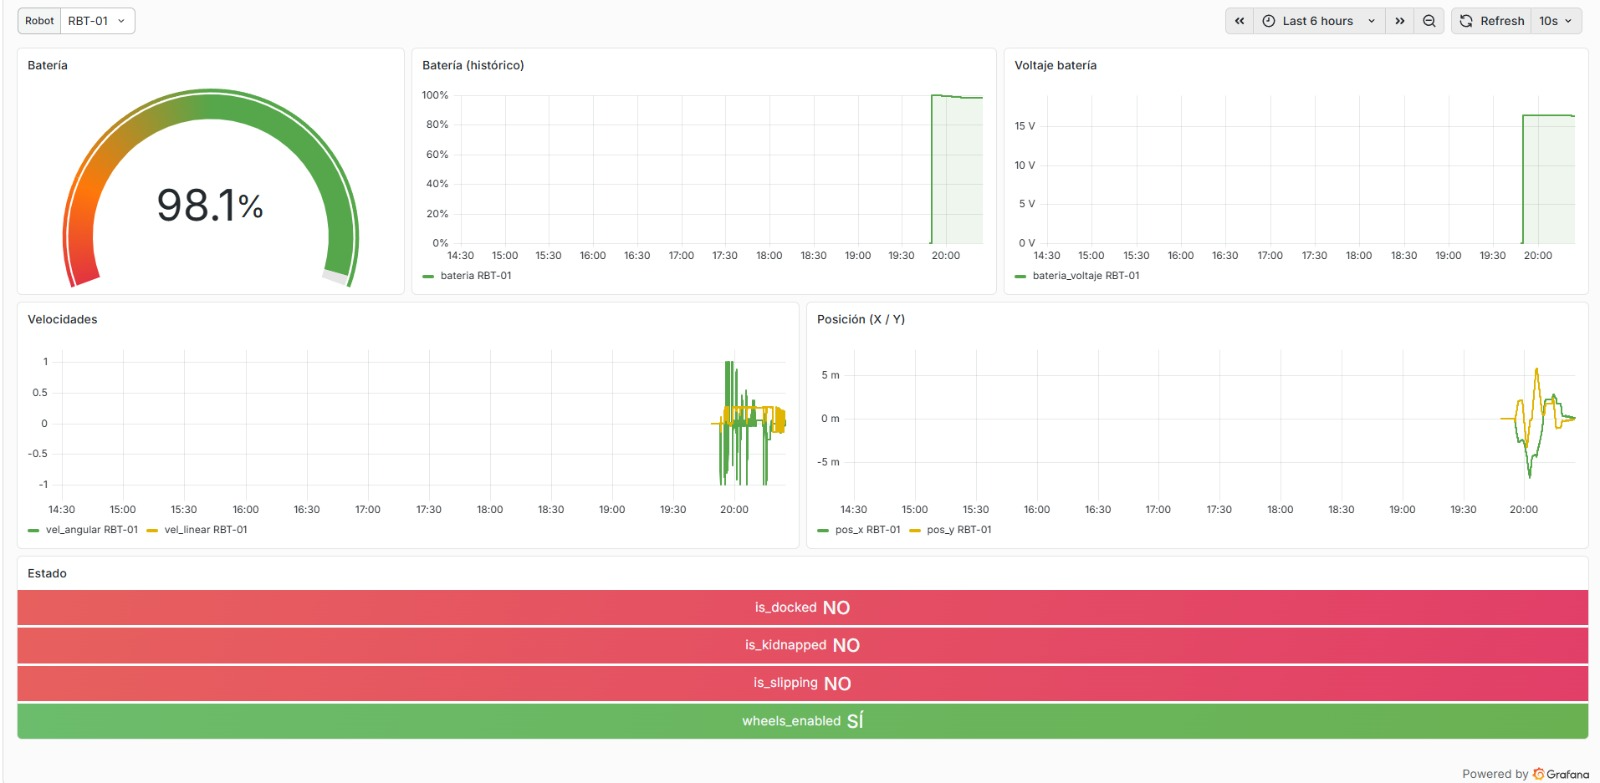
\includegraphics[width=0.9\textwidth, alt={Panel de Grafana con la telemetría del robot en tiempo real}]{recursos/figuras/grafana/dashboard.png}}
    {\fbox{\parbox[c][5cm][c]{0.9\textwidth}{\centering\itshape Captura del panel de Grafana (pendiente de incorporar en \texttt{recursos/figuras/grafana/dashboard.png}).}}}
  \caption{Panel de Grafana que visualiza la telemetría del robot en tiempo real. Fuente: elaboración propia.}
  \label{fig:grafana}
\end{figure}

\FloatBarrier

% ---------------------------------------------------------------------------
\subsection{Gestión de secretos: secret\_helper}
\label{sec:secret-helper}

El nodo \texttt{secret\_helper} centraliza la autenticación de todo el espacio de
trabajo. Aplica el patrón \gls{tofu} (\textit{trust on first use}), cuya premisa es
que el robot y el backend establecen una relación de confianza en su primer contacto
y la reutilizan en lo sucesivo: en lugar de distribuir credenciales de antemano, el
secreto se acuerda una sola vez, en el arranque inicial, y se da por fiable a partir
de entonces. En la práctica, el nodo distingue dos situaciones. Si no existe un
secreto local, ejecuta el primer arranque (\textit{first boot}): solicita un secreto
al backend con \texttt{POST /robot/\{id\}/first-boot} y lo persiste en la ruta
indicada por \texttt{SECRET\_PATH}, montada como volumen para sobrevivir a las
recreaciones del contenedor. Si el secreto ya existe, lo reutiliza para autenticarse
con \texttt{POST /robot/\{id\}/auth} y obtener un \gls{jwt}. Toda esta lógica reside en
un hilo en segundo plano (\texttt{auth\_routine}) que renueva el token de forma
proactiva: duerme una hora entre renovaciones, muy por debajo de las veinticuatro
horas de validez del \gls{jwt}, de modo que nunca se utiliza un token caducado; si una
autenticación falla, reintenta cada diez segundos. Para que el resto de nodos no tenga
que gestionar credenciales, el nodo publica el servicio \gls{ros}
\texttt{get\_robot\_token}, que devuelve el token vigente junto con un indicador de
disponibilidad (\texttt{is\_ready}); los consumidores lo invocan de forma no
bloqueante (mediante \texttt{call\_async} y un \textit{callback} de finalización) para
no detener el \textit{executor} de hilo único, y reintentan si el token todavía no
está disponible. Las figuras~\ref{fig:tofu} y~\ref{fig:token} resumen, respectivamente,
el arranque inicial con autenticación y la forma en que el resto de nodos obtienen y
emplean el token.

\begin{figure}[htbp]
  \centering
  \usetikzlibrary{arrows.meta}%
  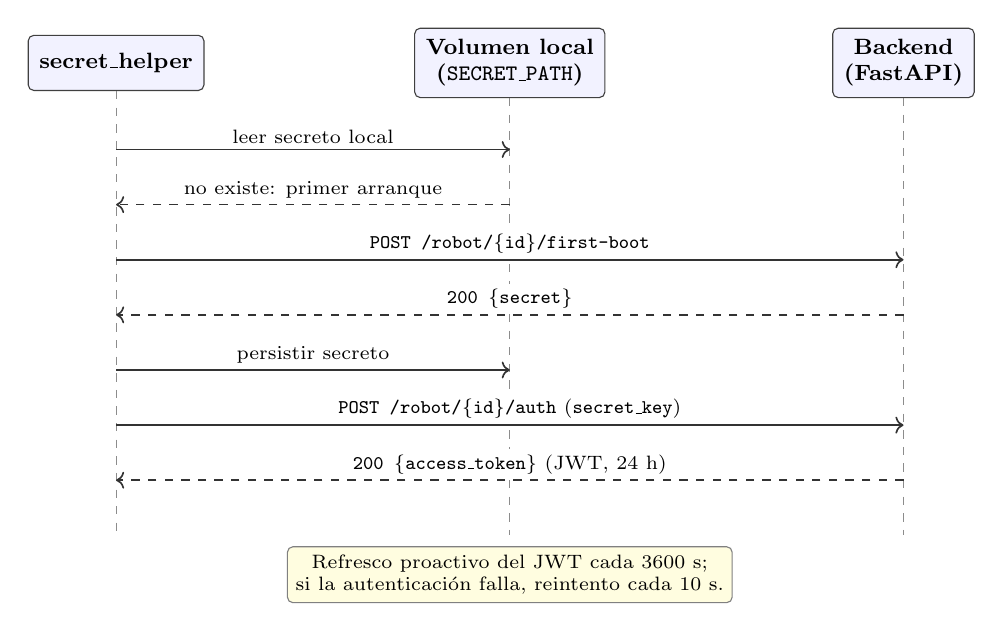
\begin{tikzpicture}[
      actor/.style={draw=black!75, rounded corners=2pt, fill=blue!5,
        font=\footnotesize\bfseries, align=center, minimum height=7mm, inner sep=4pt},
      life/.style={dashed, draw=black!45},
      msg/.style={->, line width=0.6pt, draw=black!80},
      ret/.style={->, line width=0.6pt, draw=black!80, dashed},
      etq/.style={font=\scriptsize, inner sep=2pt, fill=white},
      note/.style={draw=black!50, fill=yellow!12, rounded corners=2pt,
        font=\scriptsize, align=center, inner sep=3pt}
    ]
    \node[actor] (sh)  at (0,0)  {secret\_helper};
    \node[actor] (vol) at (5,0)  {Volumen local\\(\texttt{SECRET\_PATH})};
    \node[actor] (be)  at (10,0) {Backend\\(FastAPI)};
    \foreach \i [evaluate=\i as \yy using -0.7*\i-0.4] in {1,...,8} {
      \coordinate (r\i) at (0,\yy); }
    \draw[life] (sh.south)  -- (sh|-r8);
    \draw[life] (vol.south) -- (vol|-r8);
    \draw[life] (be.south)  -- (be|-r8);
    \draw[msg] (sh|-r1)  -- node[etq,above]{leer secreto local} (vol|-r1);
    \draw[ret] (vol|-r2) -- node[etq,above]{no existe: primer arranque} (sh|-r2);
    \draw[msg] (sh|-r3)  -- node[etq,above]{\texttt{POST /robot/\{id\}/first-boot}} (be|-r3);
    \draw[ret] (be|-r4)  -- node[etq,above]{\texttt{200 \{secret\}}} (sh|-r4);
    \draw[msg] (sh|-r5)  -- node[etq,above]{persistir secreto} (vol|-r5);
    \draw[msg] (sh|-r6)  -- node[etq,above]{\texttt{POST /robot/\{id\}/auth} (\texttt{secret\_key})} (be|-r6);
    \draw[ret] (be|-r7)  -- node[etq,above]{\texttt{200 \{access\_token\}} (JWT, 24 h)} (sh|-r7);
    \node[note] at (5,-6.5) {Refresco proactivo del JWT cada 3600 s;\\
      si la autenticación falla, reintento cada 10 s.};
  \end{tikzpicture}
  \caption[Arranque inicial y autenticación de secret\_helper]{Secuencia del
    arranque inicial (\textit{first boot}, \gls{tofu}) y la autenticación de
    \texttt{secret\_helper}: si no hay secreto local, lo solicita al backend y lo
    persiste; después lo intercambia por un \gls{jwt} que renueva de forma periódica.
    Fuente: elaboración propia.}
  \label{fig:tofu}
\end{figure}

\begin{figure}[htbp]
  \centering
  \usetikzlibrary{arrows.meta}%
  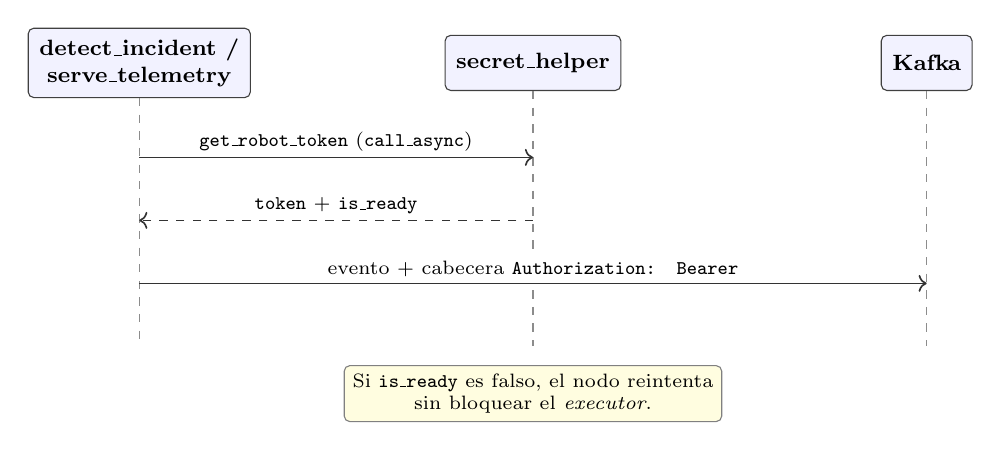
\begin{tikzpicture}[
      actor/.style={draw=black!75, rounded corners=2pt, fill=blue!5,
        font=\footnotesize\bfseries, align=center, minimum height=7mm, inner sep=4pt},
      life/.style={dashed, draw=black!45},
      msg/.style={->, line width=0.6pt, draw=black!80},
      ret/.style={->, line width=0.6pt, draw=black!80, dashed},
      etq/.style={font=\scriptsize, inner sep=2pt, fill=white},
      note/.style={draw=black!50, fill=yellow!12, rounded corners=2pt,
        font=\scriptsize, align=center, inner sep=3pt}
    ]
    \node[actor] (nodo)  at (0,0)  {detect\_incident /\\serve\_telemetry};
    \node[actor] (sh)    at (5,0)  {secret\_helper};
    \node[actor] (kafka) at (10,0) {Kafka};
    \foreach \i [evaluate=\i as \yy using -0.8*\i-0.4] in {1,...,4} {
      \coordinate (r\i) at (0,\yy); }
    \draw[life] (nodo.south)  -- (nodo|-r4);
    \draw[life] (sh.south)    -- (sh|-r4);
    \draw[life] (kafka.south) -- (kafka|-r4);
    \draw[msg] (nodo|-r1) -- node[etq,above]{\texttt{get\_robot\_token} (\texttt{call\_async})} (sh|-r1);
    \draw[ret] (sh|-r2)   -- node[etq,above]{\texttt{token} + \texttt{is\_ready}} (nodo|-r2);
    \draw[msg] (nodo|-r3) -- node[etq,above]{evento + cabecera \texttt{Authorization: Bearer}} (kafka|-r3);
    \node[note] at (5,-4.2) {Si \texttt{is\_ready} es falso, el nodo reintenta\\
      sin bloquear el \textit{executor}.};
  \end{tikzpicture}
  \caption[Obtención y uso del JWT por el resto de nodos]{Los nodos consumidores
    obtienen el \gls{jwt} del servicio \texttt{get\_robot\_token} de
    \texttt{secret\_helper} y lo adjuntan en la cabecera \texttt{Authorization: Bearer}
    de los mensajes que publican en Kafka. Fuente: elaboración propia.}
  \label{fig:token}
\end{figure}

Conviene reconocer la principal asunción de este patrón: la confianza depositada en
el primer contacto. Si un atacante se adelantara al robot legítimo y completara el
\texttt{first-boot} antes que él, podría reclamar su identidad. En el contexto de
este trabajo el riesgo se considera asumible, ya que el despliegue es local y
controlado, el aprovisionamiento del robot se realiza de forma manual en una red de
confianza y cada robot ejecuta un único \texttt{first-boot}. No obstante, el
endurecimiento de este arranque inicial queda como limitación conocida.

% =============================================================================
\section{Aplicación de usuario}
\label{sec:app-usuario}

% La plantilla no define un entorno de código para Dart; se declara aquí uno
% (dartcode) replicando el estilo de los demás listados, con el lexer 'dart'.
\newtcblisting[use counter=listing, list inside=lol, list type=listing]{dartcode}[1][]{%
  vscode-light-linenos, minted language=dart, title={Dart},
  list entry={\protect\numberline{\thelisting}Dart}, #1}
% Declarar un \newtcblisting con 'use counter=listing' dentro del documento
% reinicia \thelisting al formato plano (\arabic), deshaciendo el prefijo por
% capítulo que fija \counterwithin{listing}{chapter} en el preámbulo. Sin esta
% línea, el Índice de Códigos y las referencias perderían el prefijo (p. ej.
% «13» en lugar de «5.13», «1» en lugar de «7.1»). Se restaura aquí.
\renewcommand{\thelisting}{\thechapter.\arabic{listing}}

La aplicación con la que interactúa el usuario está desarrollada en \textit{Flutter}, lo
que permite desplegarla en múltiples plataformas (móvil, web y escritorio) desde un único
código. Esta sección describe primero su arquitectura interna y, a continuación, recorre
las pantallas que la componen, ilustradas con capturas de la aplicación en funcionamiento.

% ---------------------------------------------------------------------------
\subsection{Arquitectura de la aplicación}
\label{sec:app-arquitectura}

La aplicación separa la presentación, el estado y el acceso a datos. La comunicación con
la \gls{api} \gls{rest} se concentra en una capa de repositorios, uno por dominio
(autenticación, robots, incidencias, usuario y administración), construida sobre el
cliente \textit{dio}, que toma la dirección base del backend de \texttt{AppConfig.baseUrl}
y adjunta el \gls{jwt} de la sesión a cada petición. El estado se gestiona con
\textit{Riverpod}: controladores para el estado mutable (sesión, robots) y
\textit{providers} de tipo \textit{future} para las lecturas puntuales (perfil,
incidencias, listados de administración). Cada pantalla consume ese estado a través del
patrón \texttt{AsyncValue}, que distingue de forma uniforme los tres casos posibles
(cargando, con datos o con error) y se traduce en los componentes compartidos
\texttt{LoadingView} y \texttt{ErrorView} (este último con reintento), de modo que el
tratamiento de la carga y de los fallos es homogéneo en toda la aplicación.

La navegación se gestiona con \texttt{go\_router}, cuya función de redirección centraliza
el control de acceso en el cliente: si no hay sesión válida, cualquier ruta se redirige a
la pantalla de acceso; una vez autenticado, esa pantalla reenvía a la de inicio; y la ruta
de administración queda reservada a los usuarios con rol de administrador. El
extracto~\ref{lst:router} muestra esa lógica. El menú lateral (figura~\ref{fig:app-menu}),
común a las pantallas principales, da acceso a las secciones y a la opción de cerrar
sesión, e incorpora el conmutador de tema claro y oscuro.

\SuspendTagging{code}%
\begin{dartcode}[title={Control de acceso en el router (router.dart)}, label={lst:router}]
redirect: (context, state) {
  final isAuthRoute = state.matchedLocation == '/auth';
  // Sin sesion valida: solo se permite la pantalla de acceso.
  if (auth.status != AuthStatus.authenticated) {
    return isAuthRoute ? null : '/auth';
  }
  if (isAuthRoute) return '/home';          // Con sesion: ir a Inicio.
  // Administracion: requiere rol de administrador.
  if (state.matchedLocation == '/admin' && auth.role != 'admin') {
    return '/home';
  }
  return null;
}
\end{dartcode}%
\ResumeTagging{code}

\begin{figure}[H]
  \centering
  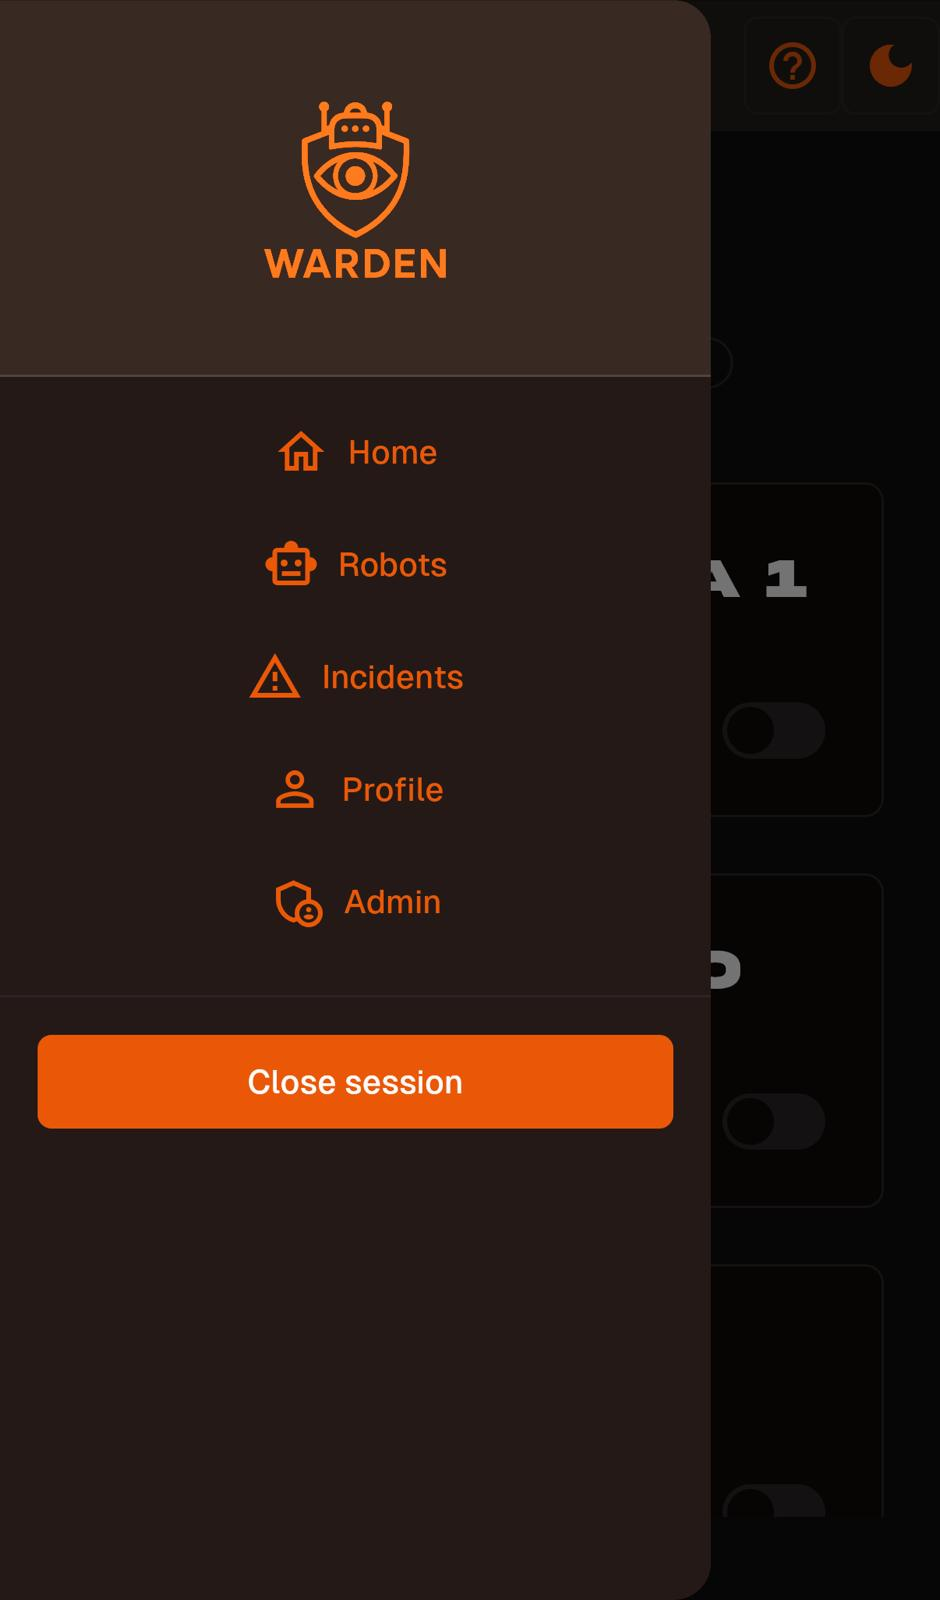
\includegraphics[width=0.30\textwidth]{recursos/figuras/app/menu.png}
  \caption[Menú de navegación de la aplicación]{Menú lateral de navegación, con acceso a
    las secciones y al cierre de sesión. Fuente: elaboración propia.}
  \label{fig:app-menu}
\end{figure}

% ---------------------------------------------------------------------------
\subsection{Recorrido por las pantallas}
\label{sec:app-pantallas}

La tabla~\ref{tab:pantallas} relaciona cada pantalla con su ruta y con los principales
endpoints del backend (tabla~\ref{tab:endpoints}) que consume. A continuación se describe
cada una.

\begin{table}[htbp]
  \centering
  \small
  \caption{Pantallas de la aplicación, su ruta y los endpoints que consumen. Fuente:
  elaboración propia.}
  \label{tab:pantallas}
  \begin{tabular}{@{}>{\raggedright\arraybackslash}p{2.5cm}
                     >{\ttfamily}l
                     >{\raggedright\arraybackslash}p{6.9cm}@{}}
    \toprule
    \textbf{Pantalla} & \textbf{\normalfont Ruta} & \textbf{Endpoints principales} \\
    \midrule
    Acceso         & /auth          & \texttt{POST /user/register}, \texttt{/user/login} \\
    \addlinespace[3pt]
    Inicio         & /home          & \texttt{GET /user/robots}; \texttt{PUT /user/\{id\}/start-patrol}, \texttt{stop-patrol} \\
    \addlinespace[3pt]
    Robots         & /robots        & \texttt{GET /user/robots}, \texttt{dashboard-url}; \texttt{POST /user/new-robot}; \texttt{PUT .../alias}, \texttt{reinstall}; \texttt{DELETE .../delete} \\
    \addlinespace[3pt]
    Incidencias    & /incidents     & \texttt{GET /user/incidents} \\
    \addlinespace[3pt]
    Detalle        & /incidents/:id & \texttt{GET /user/incidents/\{id\}/show-video} \\
    \addlinespace[3pt]
    Perfil         & /profile       & \texttt{GET /user/profile}; \texttt{PUT /user/update-info}, \texttt{update-password} \\
    \addlinespace[3pt]
    Administración & /admin         & \texttt{GET /admin/users}, \texttt{/admin/robots}; \texttt{PUT .../grant}, \texttt{revoke}; \texttt{DELETE .../delete} \\
    \bottomrule
  \end{tabular}
\end{table}

\paragraph*{Acceso.} La pantalla de acceso (figura~\ref{fig:app-acceso}) ofrece, en dos
pestañas, el inicio de sesión (correo y contraseña) y el registro de un nuevo usuario
(nombre, correo, contraseña y teléfono opcional). Un registro correcto inicia sesión de
forma automática, de modo que el usuario accede directamente a la aplicación.

\paragraph*{Inicio.} La pantalla principal, «WARDEN» (figura~\ref{fig:app-inicio}), lista
los robots del usuario con su estado de conexión y operativo, y permite iniciar o detener
la patrulla de cada uno mediante un conmutador. Un indicador general resume si el conjunto
está desarmado o asegurado. La pantalla sondea el estado real cada cinco segundos para
reflejar el \textit{heartbeat} del robot e impide detener un robot que todavía se está
configurando (mapeando), mostrando un aviso si se intenta. Ofrece además ayuda contextual
y el conmutador de tema claro y oscuro.

\paragraph*{Robots.} La pantalla de robots (figura~\ref{fig:app-robots}) gestiona el parque
de robots del usuario. Cada robot permite editar su alias, reinstalarlo (lo que borra su
mapa y reinicia el ciclo, con confirmación previa), abrir su panel de telemetría en Grafana
y eliminarlo. El alta de un robot se realiza mediante un diálogo que solicita su
identificador y un alias.

\paragraph*{Incidencias y detalle.} El listado de incidencias
(figura~\ref{fig:app-incidencias}) muestra cada suceso con un identificador abreviado, el
robot que lo originó, la fecha y su estado (revisado o pendiente). Al abrir el detalle, la
aplicación reproduce el clip de vídeo asociado mediante un reproductor incrustado que carga
la \acrshort{url} prefirmada de MinIO, con repliegue a la apertura en el navegador si la
reproducción falla. El detalle ofrece además un acceso directo para avisar a las
autoridades.

\paragraph*{Perfil.} La pantalla de perfil (figura~\ref{fig:app-perfil}) permite consultar
y editar los datos personales del usuario, así como cambiar la contraseña, en dos
formularios independientes.

\paragraph*{Administración.} Disponible solo para administradores, el panel de
administración (figura~\ref{fig:app-admin}) se organiza en tres pestañas: usuarios, donde
se conceden o revocan privilegios de administrador y se eliminan cuentas; robots, donde se
listan y eliminan los robots del sistema; e incidencias, donde se consultan las de un robot
concreto a partir de su identificador.

Las figuras~\ref{fig:app-acceso} a~\ref{fig:app-admin} recogen las capturas de las
pantallas descritas, en el mismo orden en que se han presentado.

\begin{figure}[H]
  \centering
  \begin{subfigure}[t]{0.32\textwidth}
    \centering
    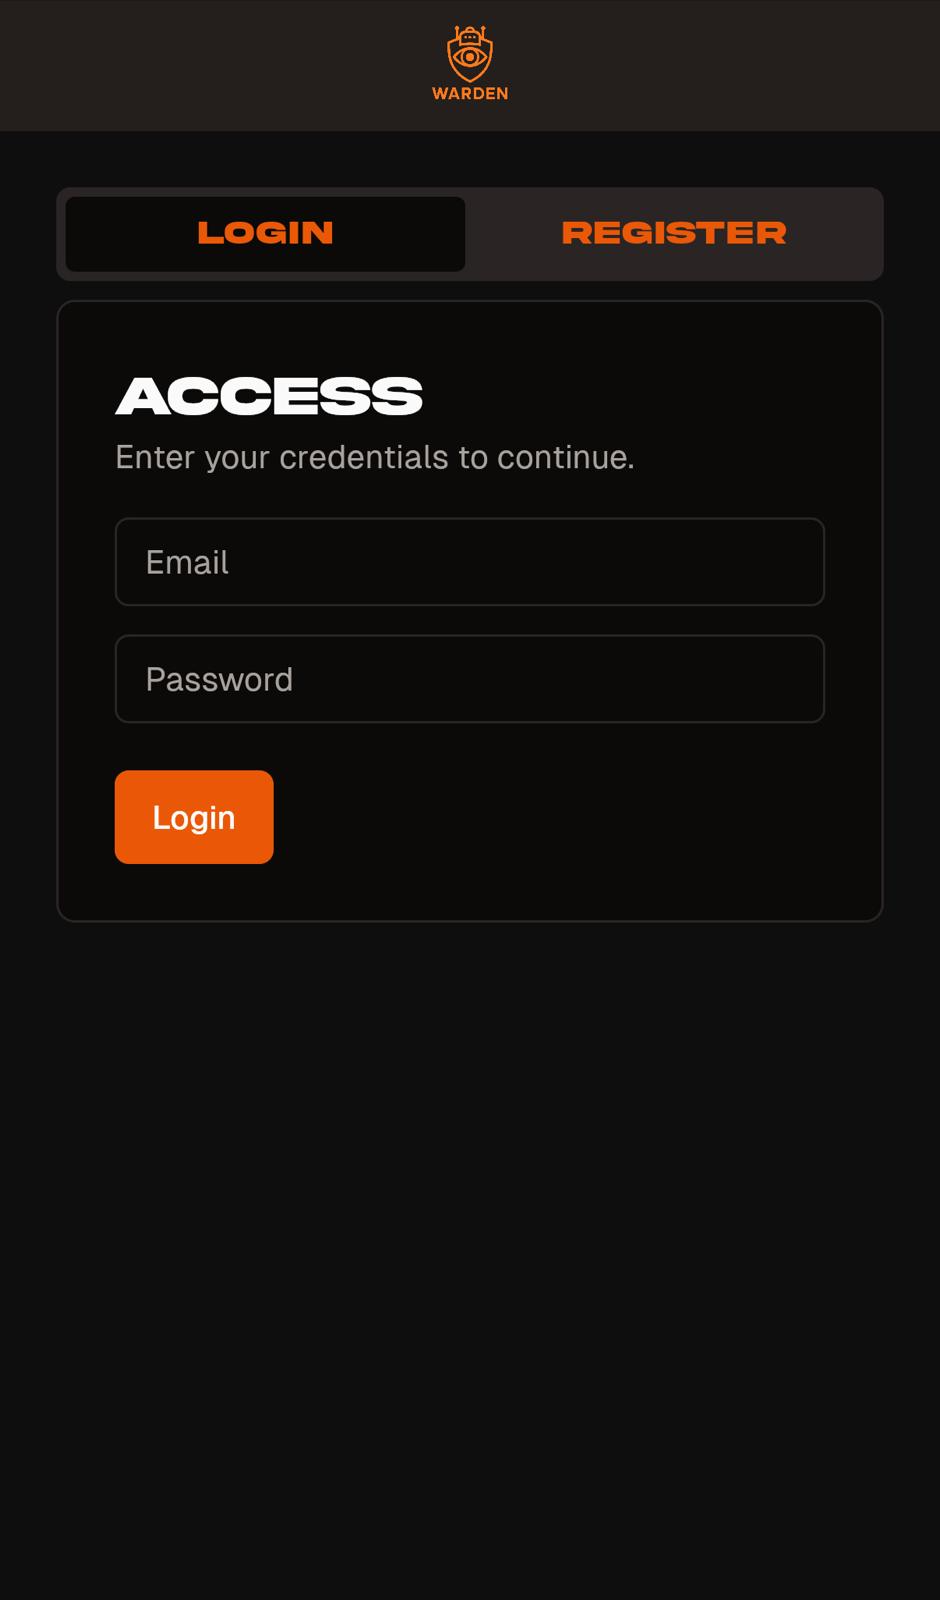
\includegraphics[width=\linewidth]{recursos/figuras/app/login.png}
    \caption{Inicio de sesión.}
    \label{fig:app-login}
  \end{subfigure}
  \hfill
  \begin{subfigure}[t]{0.32\textwidth}
    \centering
    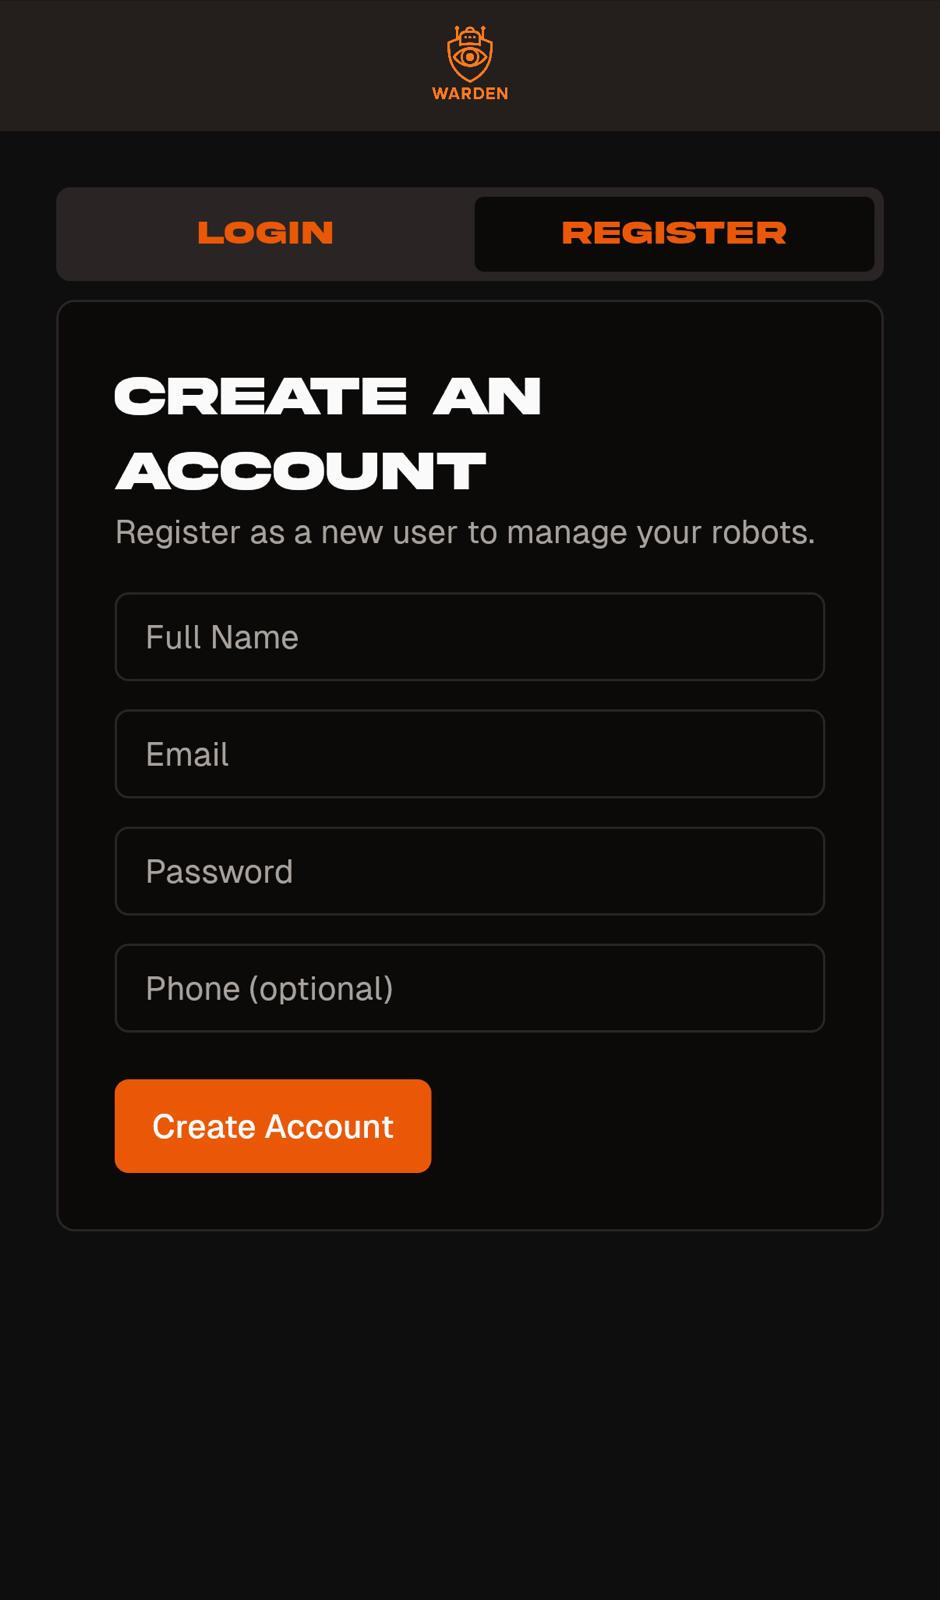
\includegraphics[width=\linewidth]{recursos/figuras/app/register.png}
    \caption{Registro de usuario.}
    \label{fig:app-register}
  \end{subfigure}
  \caption[Pantalla de acceso]{Pantalla de acceso, con las pestañas de inicio de sesión y
    registro. Fuente: elaboración propia.}
  \label{fig:app-acceso}
\end{figure}

\begin{figure}[H]
  \centering
  \begin{subfigure}[t]{0.32\textwidth}
    \centering
    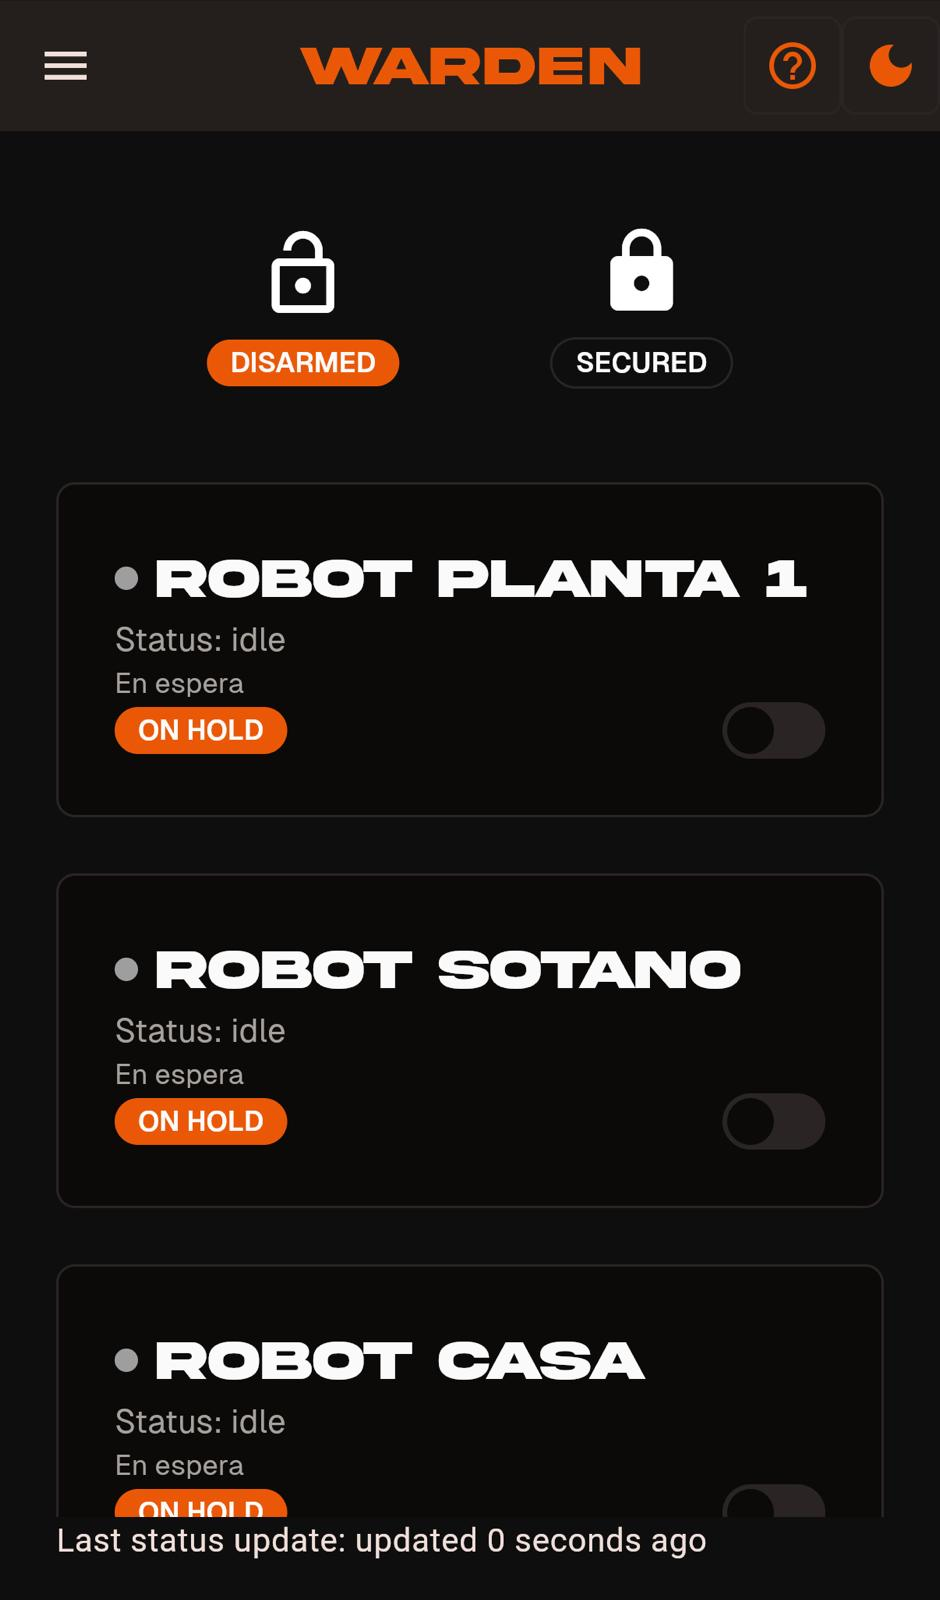
\includegraphics[width=\linewidth]{recursos/figuras/app/home.png}
    \caption{Lista de robots y estado.}
    \label{fig:app-home}
  \end{subfigure}
  \hfill
  \begin{subfigure}[t]{0.32\textwidth}
    \centering
    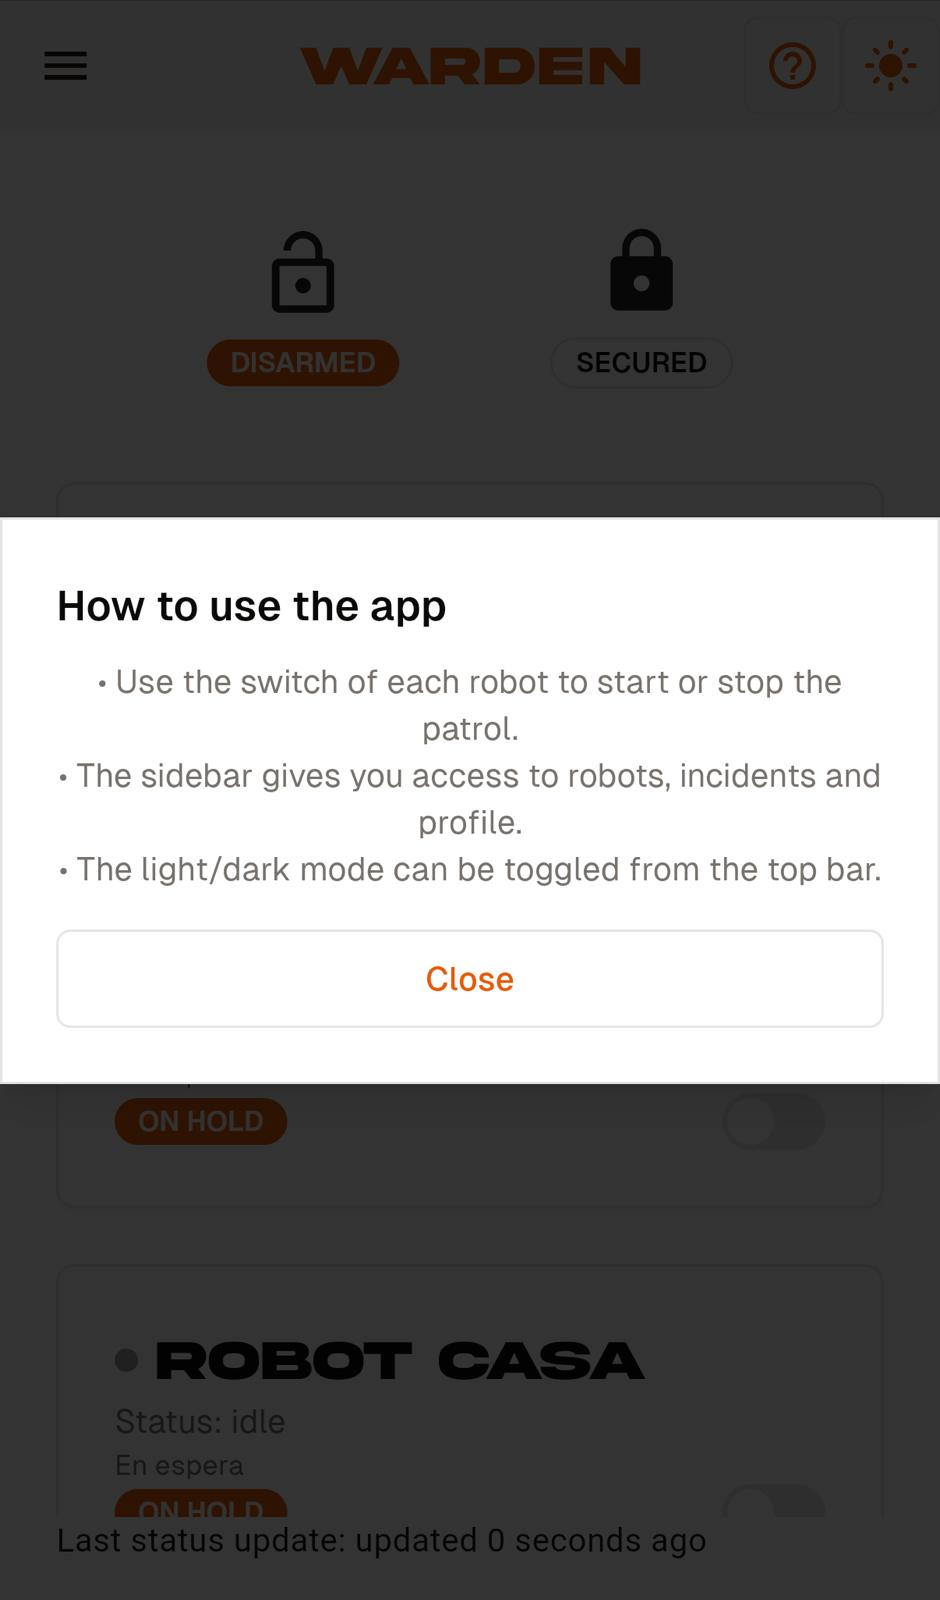
\includegraphics[width=\linewidth]{recursos/figuras/app/howto-light.png}
    \caption{Ayuda contextual (tema claro).}
    \label{fig:app-howto}
  \end{subfigure}
  \caption[Pantalla de inicio]{Pantalla de inicio: lista de robots con control de patrulla
    (a) y ayuda contextual en tema claro (b). Fuente: elaboración propia.}
  \label{fig:app-inicio}
\end{figure}

\begin{figure}[H]
  \centering
  \begin{subfigure}[t]{0.32\textwidth}
    \centering
    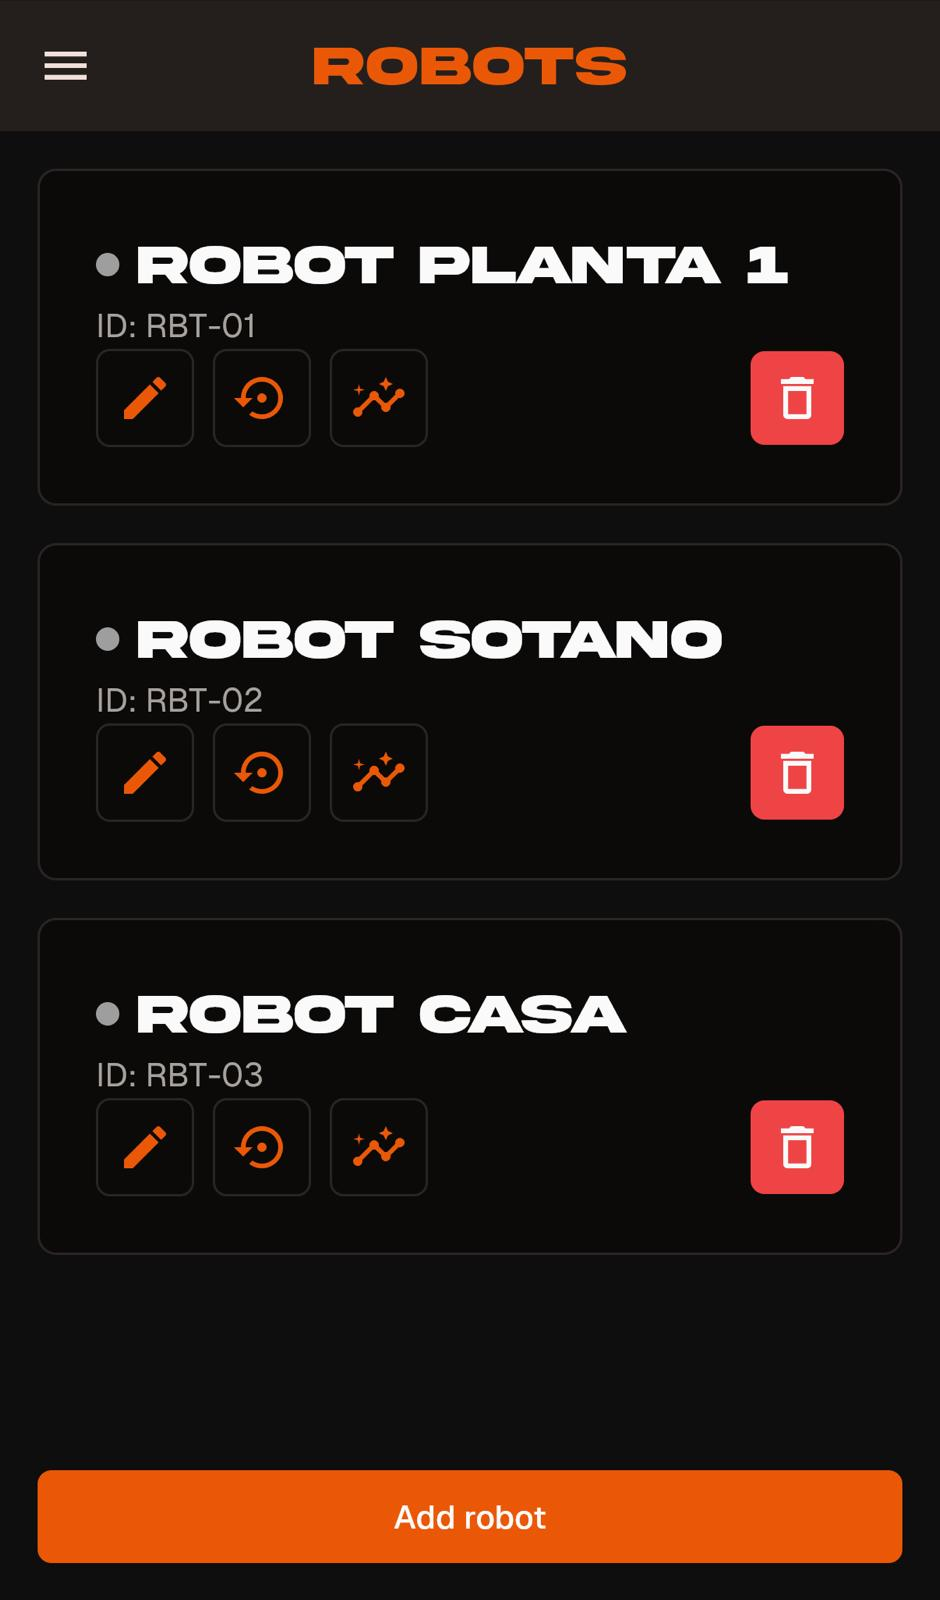
\includegraphics[width=\linewidth]{recursos/figuras/app/robots.png}
    \caption{Parque de robots.}
    \label{fig:app-robots-lista}
  \end{subfigure}
  \hfill
  \begin{subfigure}[t]{0.32\textwidth}
    \centering
    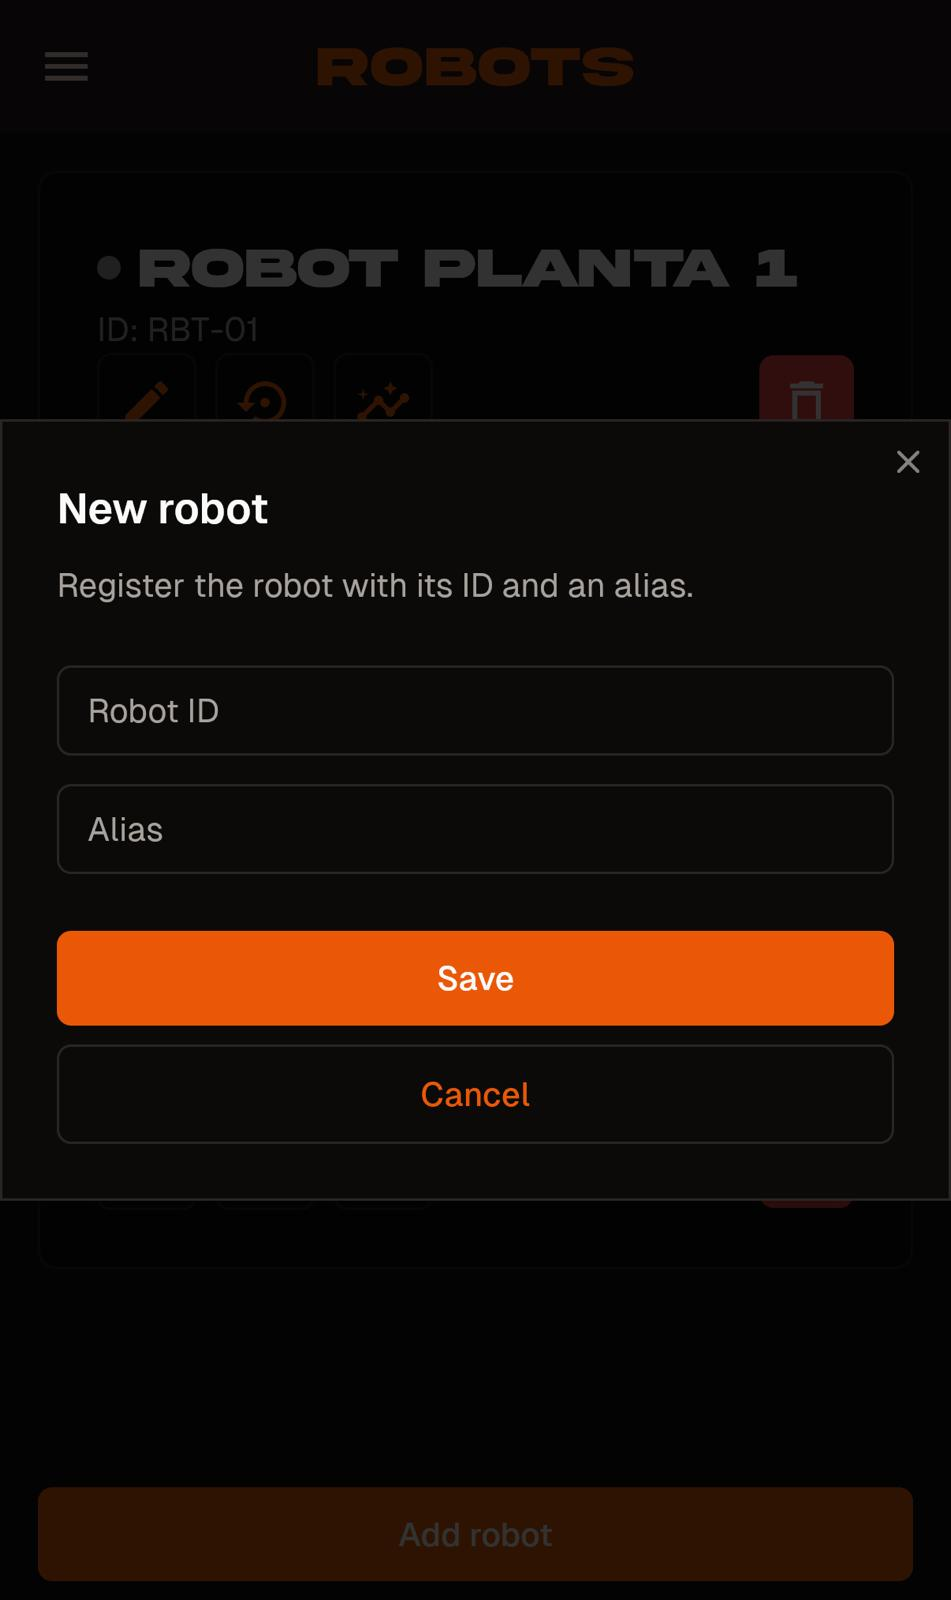
\includegraphics[width=\linewidth]{recursos/figuras/app/new-robot.png}
    \caption{Alta de un robot.}
    \label{fig:app-newrobot}
  \end{subfigure}
  \caption[Pantalla de gestión de robots]{Gestión del parque de robots (a) y diálogo de
    alta (b). Fuente: elaboración propia.}
  \label{fig:app-robots}
\end{figure}

\begin{figure}[H]
  \centering
  \begin{subfigure}[t]{0.32\textwidth}
    \centering
    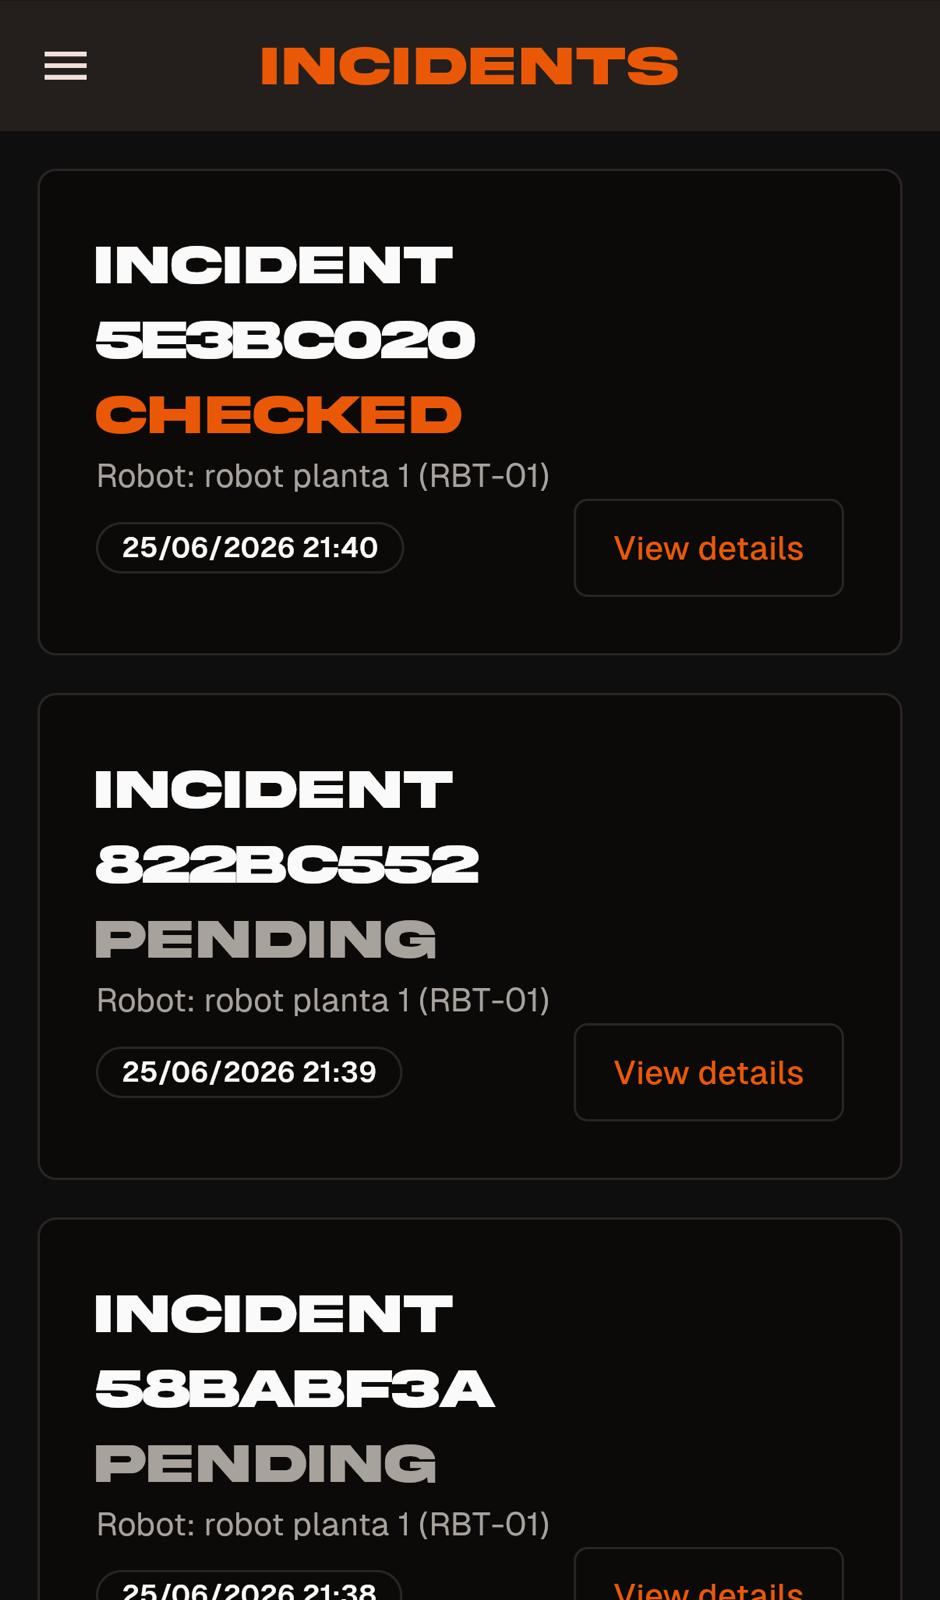
\includegraphics[width=\linewidth]{recursos/figuras/app/incidents.png}
    \caption{Listado de incidencias.}
    \label{fig:app-incidents}
  \end{subfigure}
  \hfill
  \begin{subfigure}[t]{0.32\textwidth}
    \centering
    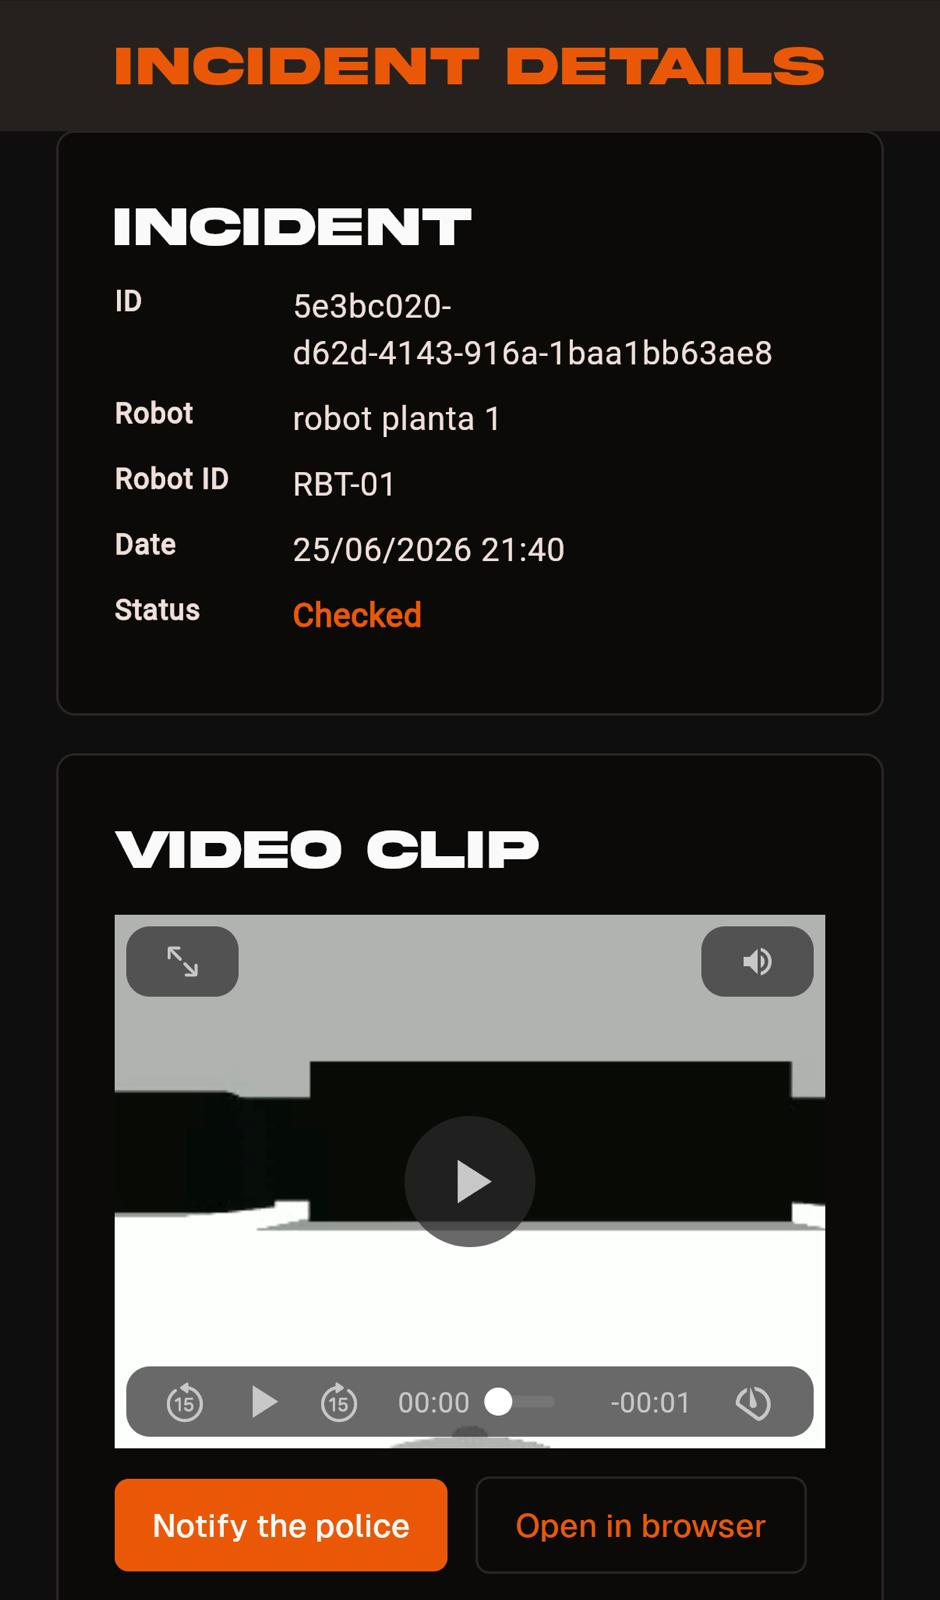
\includegraphics[width=\linewidth]{recursos/figuras/app/incident-details.png}
    \caption{Detalle con reproducción del vídeo.}
    \label{fig:app-incident-detail}
  \end{subfigure}
  \caption[Pantalla de incidencias]{Listado de incidencias (a) y detalle con el clip de
    vídeo (b). Fuente: elaboración propia.}
  \label{fig:app-incidencias}
\end{figure}

\begin{figure}[H]
  \centering
  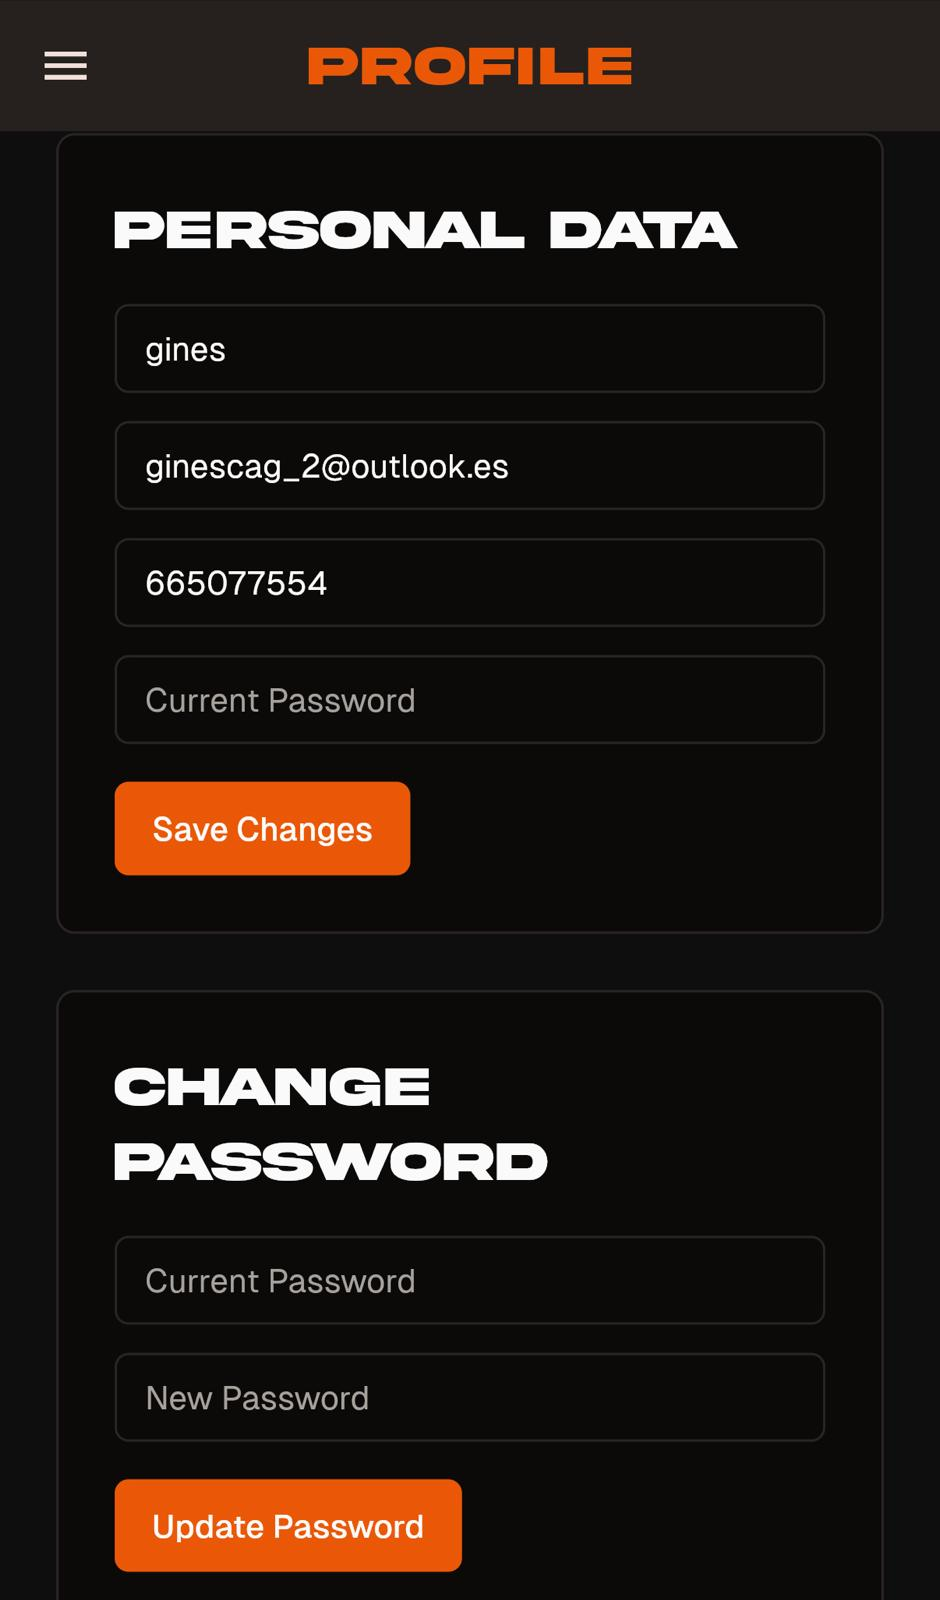
\includegraphics[width=0.30\textwidth]{recursos/figuras/app/profile.png}
  \caption[Pantalla de perfil]{Pantalla de perfil, con la edición de datos personales y el
    cambio de contraseña. Fuente: elaboración propia.}
  \label{fig:app-perfil}
\end{figure}

\begin{figure}[H]
  \centering
  \begin{subfigure}[t]{0.31\textwidth}
    \centering
    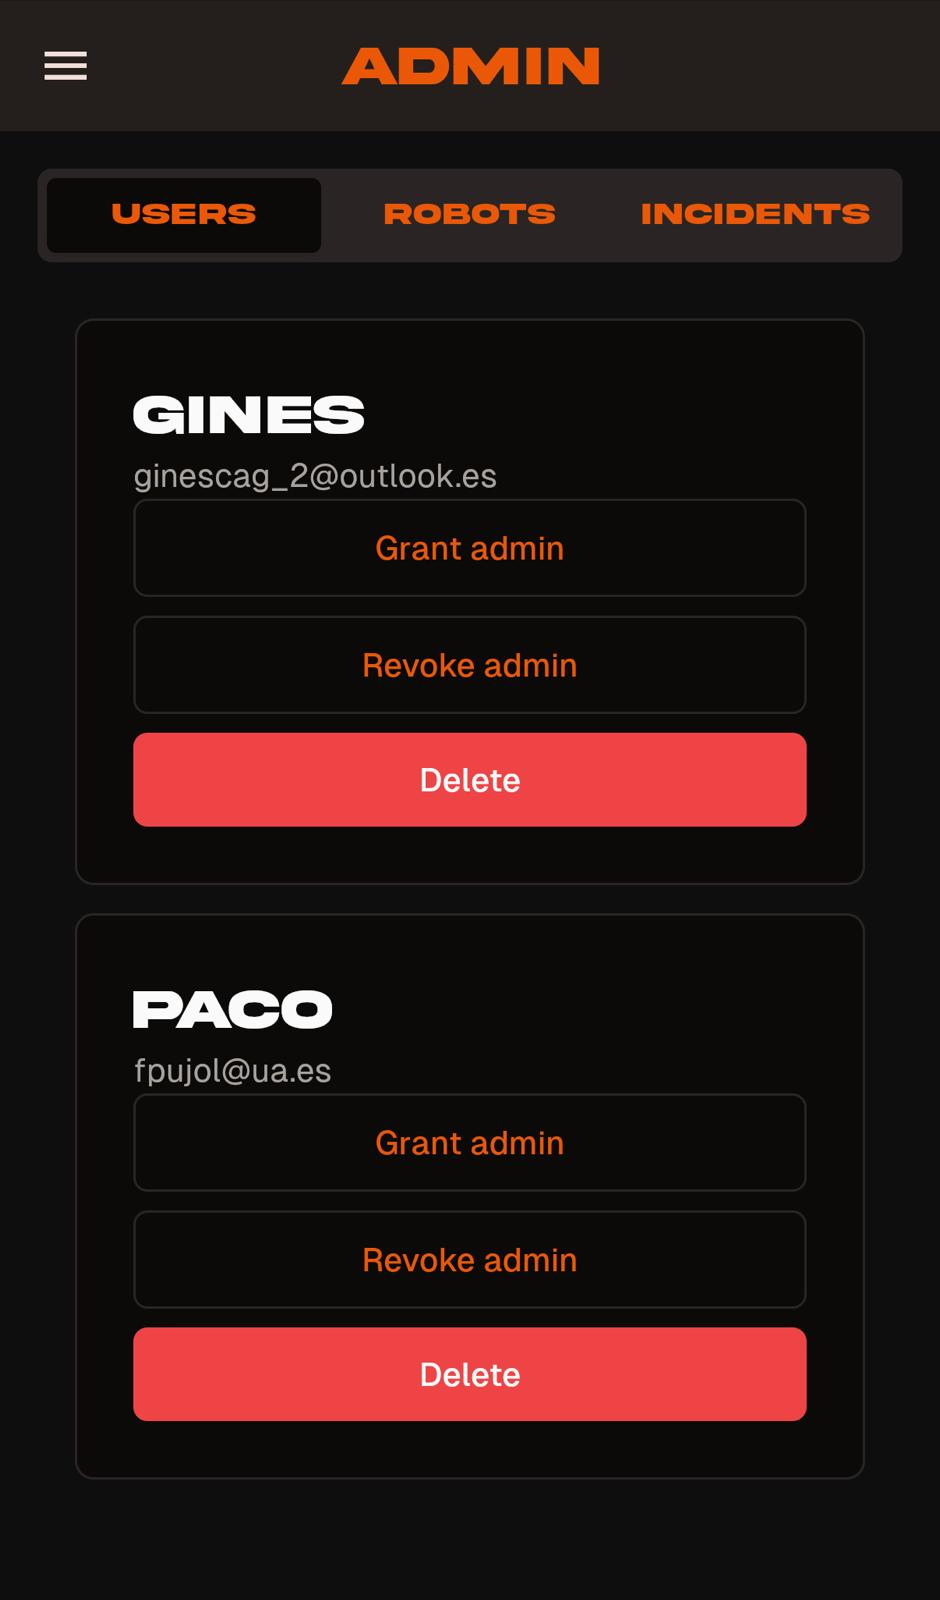
\includegraphics[width=\linewidth]{recursos/figuras/app/admin-users.png}
    \caption{Usuarios.}
    \label{fig:app-admin-users}
  \end{subfigure}
  \hfill
  \begin{subfigure}[t]{0.31\textwidth}
    \centering
    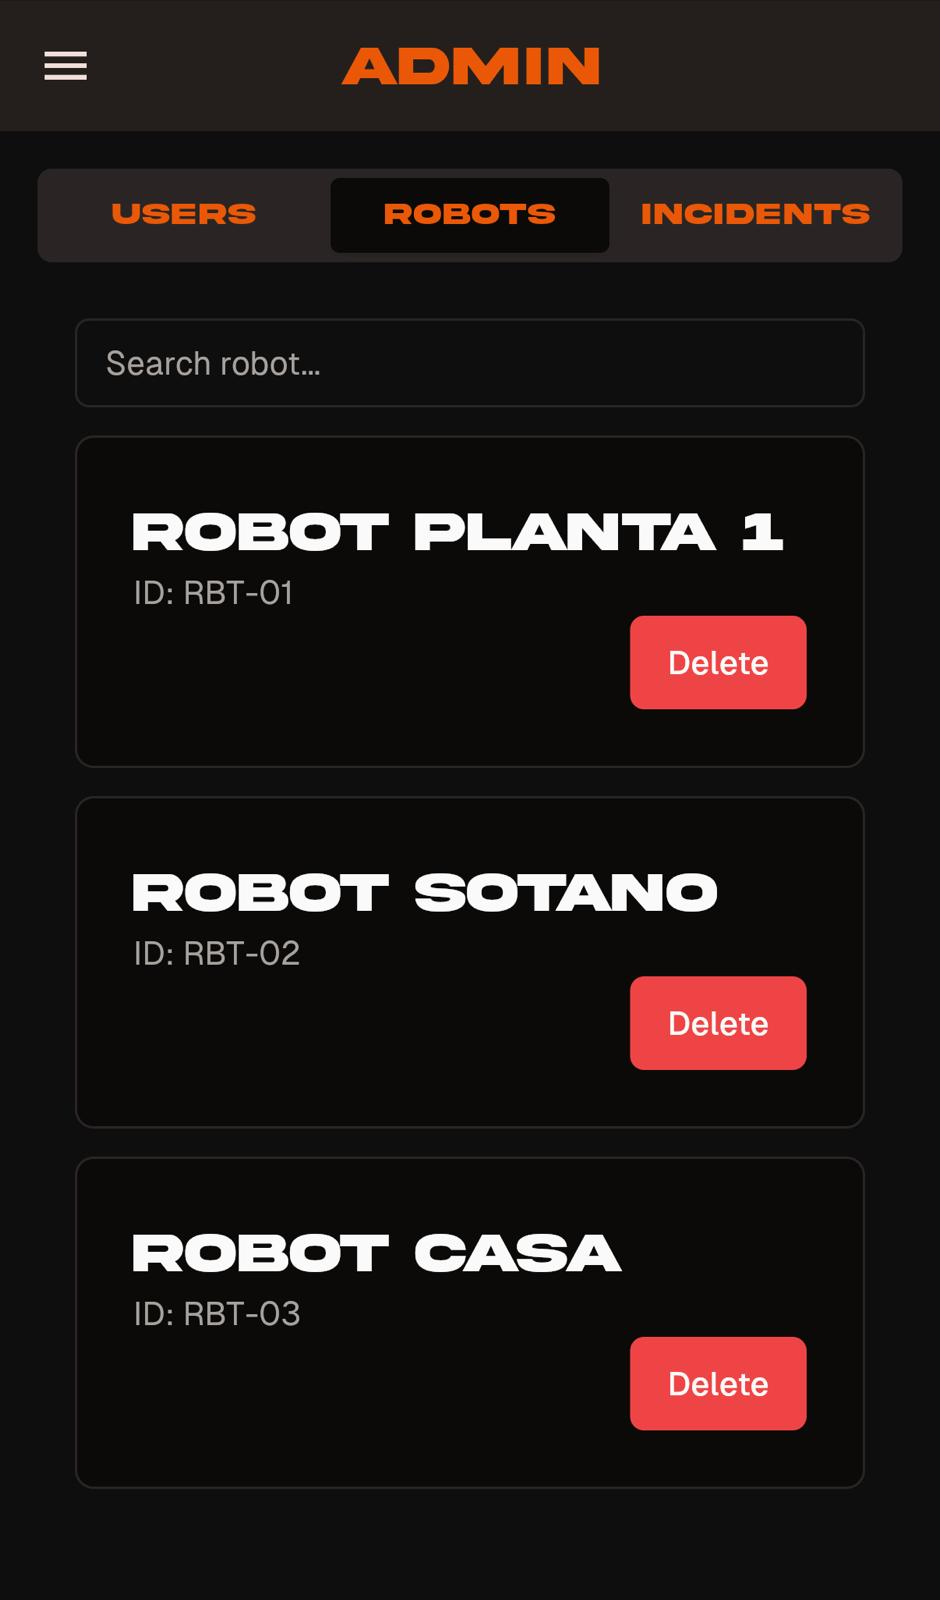
\includegraphics[width=\linewidth]{recursos/figuras/app/admin-robots.png}
    \caption{Robots.}
    \label{fig:app-admin-robots}
  \end{subfigure}
  \hfill
  \begin{subfigure}[t]{0.31\textwidth}
    \centering
    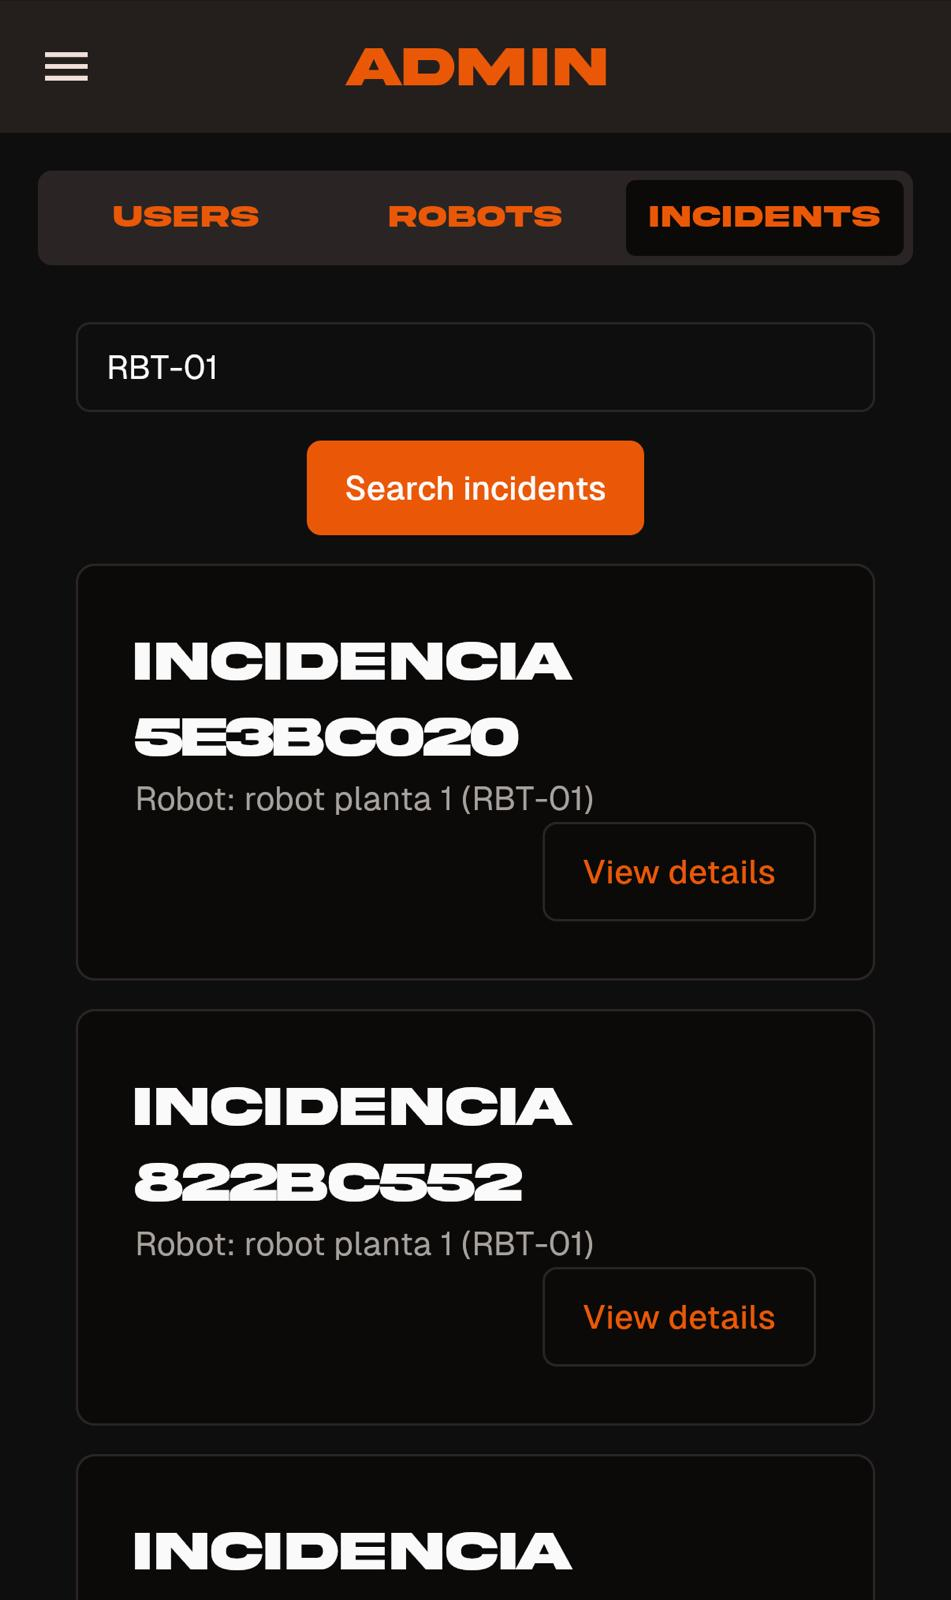
\includegraphics[width=\linewidth]{recursos/figuras/app/admin-incidents.png}
    \caption{Incidencias por robot.}
    \label{fig:app-admin-incidents}
  \end{subfigure}
  \caption[Panel de administración]{Panel de administración: gestión de usuarios (a),
    robots (b) e incidencias por robot (c). Fuente: elaboración propia.}
  \label{fig:app-admin}
\end{figure}

\FloatBarrier

Con la descripción de la aplicación de usuario se completa el recorrido por las capas del
sistema, desde la infraestructura hasta la interfaz con la que opera el usuario. El
Capítulo~\ref{cap:resultados} aborda la validación del conjunto: el alcance de las pruebas
realizadas, el escenario previsto y el estado actual de la evaluación.
